\clearpage
\section*{CHƯƠNG 7. THIẾT KẾ CHI TIẾT KIẾN TRÚC PHẦN CỨNG}
\addcontentsline{toc}{section}{\numberline{}CHƯƠNG 7. THIẾT KẾ CHI TIẾT KIẾN TRÚC PHẦN CỨNG}
\setcounter{section}{7}
\setcounter{subsection}{0}
\setcounter{figure}{0}
\setcounter{table}{0}

\subsection{Các khối chức năng của bộ mã hóa/giải mã Chaos-based}

Hệ thống mật mã hình ảnh dựa trên hệ hỗn loạn được  nghiên cứu thiết kế tuân theo cấu trúc mạng hoán vị - thay thế đặc trưng, bao gồm hai khâu xử lý cốt lõi: Xáo trộn (Confusion) và Khuếch tán (Diffusion), nhận dữ liệu để mã hoá thông qua bộ sinh hỗn loạn PLCM.

Để đáp ứng yêu cầu linh hoạt của hệ thống, thiết kế được phân tách thành hai khía cạnh: Mô hình luồng dữ liệu thuật toán và Mô hình kiến trúc phần cứng triển khai.

\subsubsection{Mô hình luồng dữ liệu thuật toán}

Hệ thống hoạt động dưới hai chế độ độc lập là mã hóa và giải mã, được định tuyến linh hoạt thông qua tín hiệu điều khiển \texttt{mode}. Để đảm bảo hiệu ứng tuyết lở và đạt được mức độ an toàn mật mã cao nhất, cả hai chế độ này đều yêu cầu dữ liệu phải trải qua quá trình xử lý lặp lại 5 vòng ($r=5$).

Ở chế độ mã hóa, luồng dữ liệu đầu vào bao gồm chuỗi 25 byte hệ số DC được trích xuất từ gói NALU sẽ được đưa vào khối xáo trộn \texttt{confusion} trước tiên. Quá trình này sử dụng phép hoán vị Arnold's Cat Map để phá vỡ hoàn toàn trật tự ban đầu của chuỗi dữ liệu. Ngay sau đó, dữ liệu tiếp tục đi qua khối khuếch tán \texttt{diffusion} để thực hiện phép toán XOR nhằm biến đổi triệt để giá trị của từng byte. Trong toàn bộ chu trình này, khối \texttt{plcm} đóng vai trò cốt lõi khi liên tục cung cấp các tham số hoán vị động $p$ và $q$ cho khối xáo trộn, đồng thời sinh ra chuỗi khóa giả ngẫu nhiên cấp cho khối khuếch tán.

\begin{figure}[H]
	\centering
	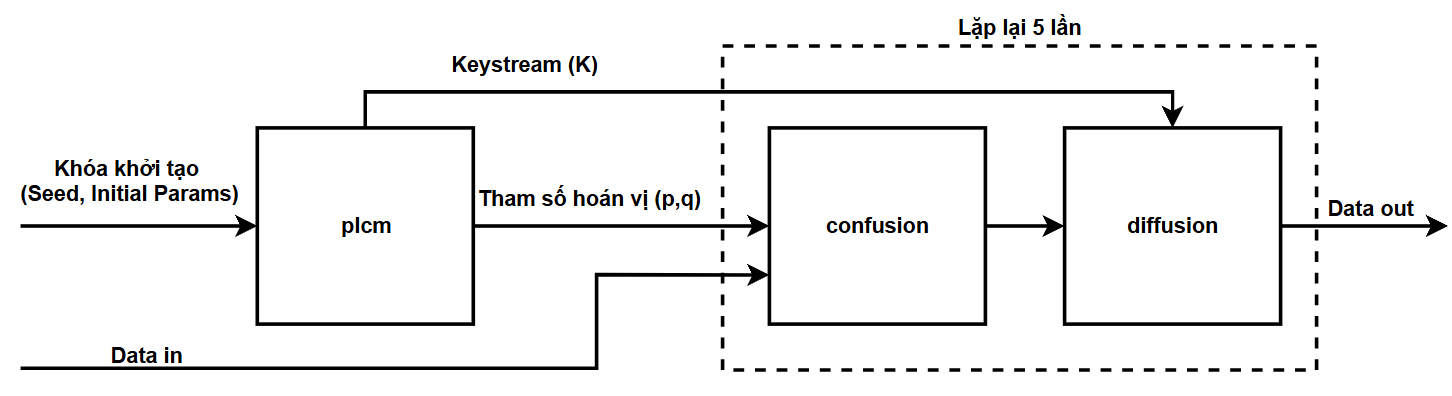
\includegraphics[width=1\textwidth]{Figures/mahoa.png}
	\caption{Sơ đồ thuật toán luồng Mã hóa}
	\label{fig:mahoa}
\end{figure}

Ngược lại, ở chế độ giải mã, luồng dữ liệu được xử lý theo nguyên lý nghịch đảo toán học. Cụ thể, dữ liệu bản mã sẽ đi qua khối khuếch tán \texttt{diffusion} trước để giải trừ nhiễu thông qua phép toán XOR với chuỗi khóa giả ngẫu nhiên. Sau khi khôi phục được giá trị, dữ liệu mới được đưa qua khối xáo trộn \texttt{confusion}, sử dụng ma trận Arnold's Cat Map nghịch đảo để sắp xếp các phần tử về đúng trật tự nguyên bản.

\begin{figure}[H]
	\centering
	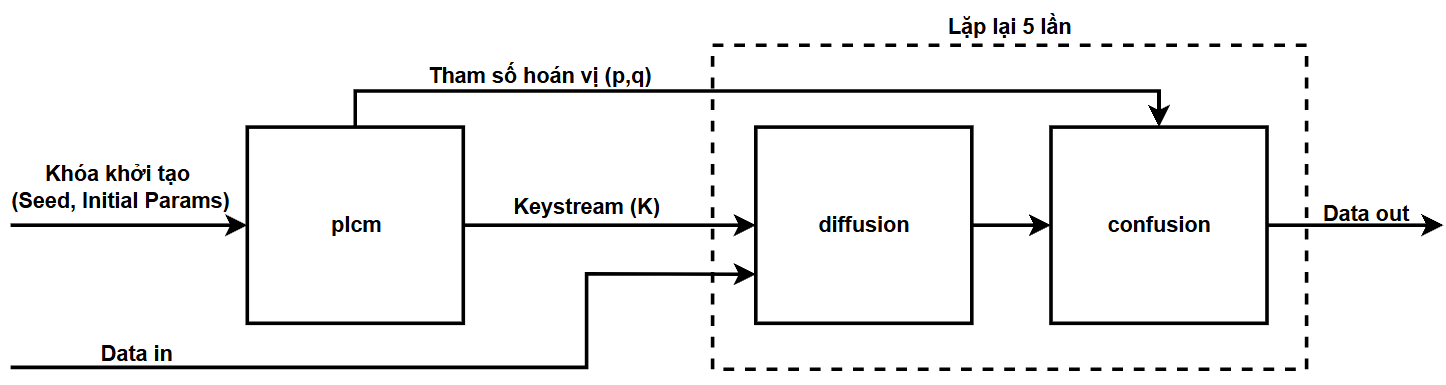
\includegraphics[width=1\textwidth]{Figures/giaima.png}
	\caption{Sơ đồ thuật toán luồng Giải mã}
	\label{fig:giaima}
\end{figure}

\subsubsection{Mô hình kiến trúc phần cứng}

Về mặt triển khai vật lý, mặc dù thuật toán yêu cầu luồng dữ liệu đi qua các khối toán học theo một trình tự nhất định, việc ghép nối trực tiếp đầu ra của khối này vào đầu vào của khối kia sẽ gây lãng phí tài nguyên nghiêm trọng, đặc biệt khi hệ thống phải thực thi lặp lại tới 5 vòng. Để khắc phục vấn đề này, phần cứng được thiết kế theo kiến trúc máy trạng thái kết hợp đường dẫn dữ liệu (FSMD), hoạt động đồng bộ với cơ chế điều phối qua một bộ nhớ trung tâm.

\begin{figure}[H]
	\centering
	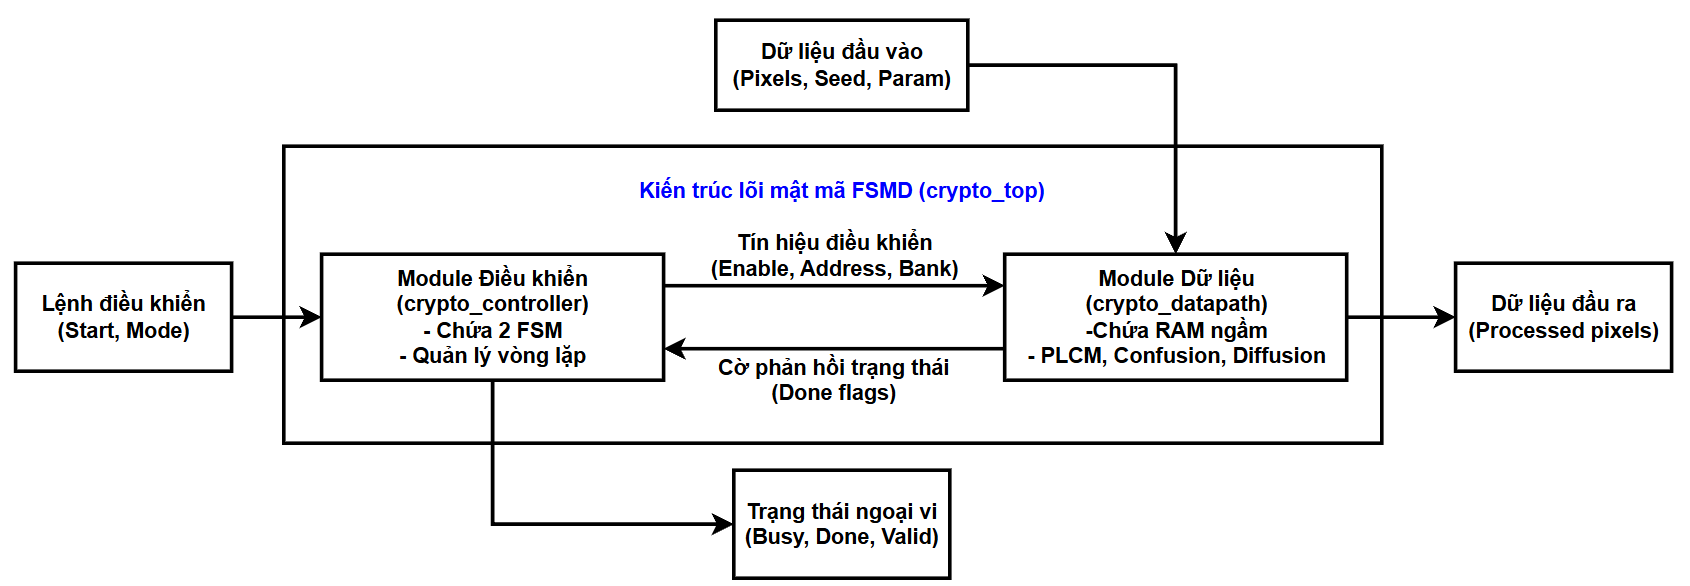
\includegraphics[width=1\textwidth]{Figures/fsmd.png}
	\caption{Sơ đồ khối kiến trúc FSMD cấp hệ thống}
	\label{fig:fsmd}
\end{figure}

Kiến trúc phần cứng này mang lại nhiều ưu điểm vượt trội nhờ khả năng phân tách rõ ràng giữa phân hệ điều khiển và phân hệ dữ liệu. Trong đó, máy trạng thái trung tâm \texttt{crypto\_controller} chịu trách nhiệm phát ra các tín hiệu điều khiển nhằm cấu hình mạng lưới bộ ghép kênh. Khối đường dẫn dữ liệu \texttt{crypto\_datapath} đóng vai trò thực thi, chỉ chứa các cỗ máy toán học và bộ nhớ RAM nội bộ. Sự phân tách này cho phép hệ thống dễ dàng chuyển đổi qua lại giữa luồng mã hóa và giải mã chỉ bằng cách thay đổi trạng thái của tín hiệu \texttt{mode} mà không cần phải can thiệp hay thay đổi các kết nối vật lý.

Bên cạnh đó, để tối ưu hóa thiết kế khi triển khai trên nền tảng FPGA, hệ thống không tiến hành xử lý song song toàn bộ khung hình video cùng lúc. Thay vào đó, dữ liệu hệ số DC được nạp vào dưới dạng một luồng bit nối tiếp một chiều. Phần cứng sẽ tự động cuộn chuỗi này thành một ma trận ảo hai chiều kích thước $5 \times 5$ (tương đương 25 byte) để xử lý tuần tự, qua đó giúp thu nhỏ tối đa kích thước của các mảng thanh ghi.

Đặc biệt, hệ thống áp dụng triệt để kỹ thuật tái sử dụng phần cứng bằng cách chỉ khởi tạo duy nhất một lõi xáo trộn \texttt{confusion} và một lõi khuếch tán \texttt{diffusion}. Trong suốt 5 vòng lặp của thuật toán, dữ liệu được liên tục đọc ra và ghi đè trở lại vào các mảng bộ nhớ \texttt{data\_ram} và \texttt{temp\_ram}. Hướng thiết kế này đánh đổi một phần tốc độ thông lượng nhưng bù lại lại tối ưu hơn về mặt tài nguyên logic, đem lại sự cân bằng giữa tốc độ và tài nguyên phần cứng.

\subsection{Đặc tả chi tiết các khối con}
\subsubsection{Khối crypto\_top}
\textbf{Đặc tả chức năng hoạt động} 

Khối \texttt{crypto\_top} đóng vai trò là lõi IP mức cao nhất trong quy trình thiết kế phần cứng của hệ thống mật mã. Đặc điểm nổi bật của khối này là thiết kế thuần cấu trúc và mang tính chất thụ động. Bản thân \texttt{crypto\_top} không chứa máy trạng thái hữu hạn (FSM) hay các mạch tổ hợp tính toán độc lập, mà chỉ đóng vai trò là lớp vỏ bọc nhằm định tuyến tín hiệu và kết nối hai phân hệ chính: khối điều khiển \texttt{crypto\_controller} và khối đường dẫn dữ liệu \texttt{crypto\_datapath}.

Nhiệm vụ trọng tâm của khối là phân bổ tín hiệu giao tiếp ngoại vi một cách tối ưu. Cụ thể, các tín hiệu mang tính chất điều khiển tiến trình như \texttt{start\_system} và \texttt{pixel\_in\_valid} được dẫn trực tiếp vào khối \texttt{crypto\_controller} để đồng bộ hóa hoạt động của các máy trạng thái. Trong khi đó, các bus dữ liệu kích thước lớn bao gồm \texttt{seed\_x}, \texttt{param\_p} và chuỗi điểm ảnh \texttt{pixel\_in} được kết nối thẳng đến \texttt{crypto\_datapath} để ghi trực tiếp vào các mảng RAM nội bộ, qua đó giúp tối ưu hóa đường truyền và giảm tải đáng kể cho khối điều khiển.

Ở chiều phản hồi, các cờ báo hiệu tiến độ hoàn thành từ phân hệ dữ liệu (\texttt{plcm\_done}, \texttt{conf\_done}, \texttt{diff\_done}) được đưa ngược về phân hệ điều khiển để làm điều kiện chuyển đổi trạng thái. Sự phối hợp nhịp nhàng giữa các luồng tín hiệu này tạo nên một kiến trúc điều khiển kết hợp dữ liệu (FSMD) khép kín, hoạt động đồng bộ và tối ưu hóa tài nguyên phần cứng trên vi mạch.

\textbf{Các tín hiệu vào/ra}

Giao diện của lõi IP được quy hoạch theo tiêu chuẩn thiết kế chung nhằm đảm bảo khả năng tích hợp linh hoạt với các vi điều khiển hoặc các hệ thống SoC bên ngoài. Các tín hiệu giao tiếp được chia thành các nhóm chức năng rõ ràng: nhóm xung nhịp (\texttt{clk}) và đặt lại hệ thống (\texttt{rst\_n}), nhóm lệnh kích hoạt (\texttt{start\_system}) và cấu hình chiều hoạt động (\texttt{mode}), cùng nhóm các vector thông số khởi tạo 64-bit cho các phân hệ hỗn loạn. Đối với quá trình truyền nhận, hệ thống sử dụng các kênh dữ liệu tuần tự 8-bit (\texttt{pixel\_in}, \texttt{pixel\_out}) kèm theo cờ xác nhận tính hợp lệ (\texttt{valid}), kết hợp với cờ báo bận (\texttt{system\_busy}) và cờ hoàn thành (\texttt{system\_done}) để thiết bị ngoại vi dễ dàng nắm bắt trạng thái hoạt động của lõi mật mã.

\textbf{Sơ đồ khối}

\begin{figure}[H]
	\centering
	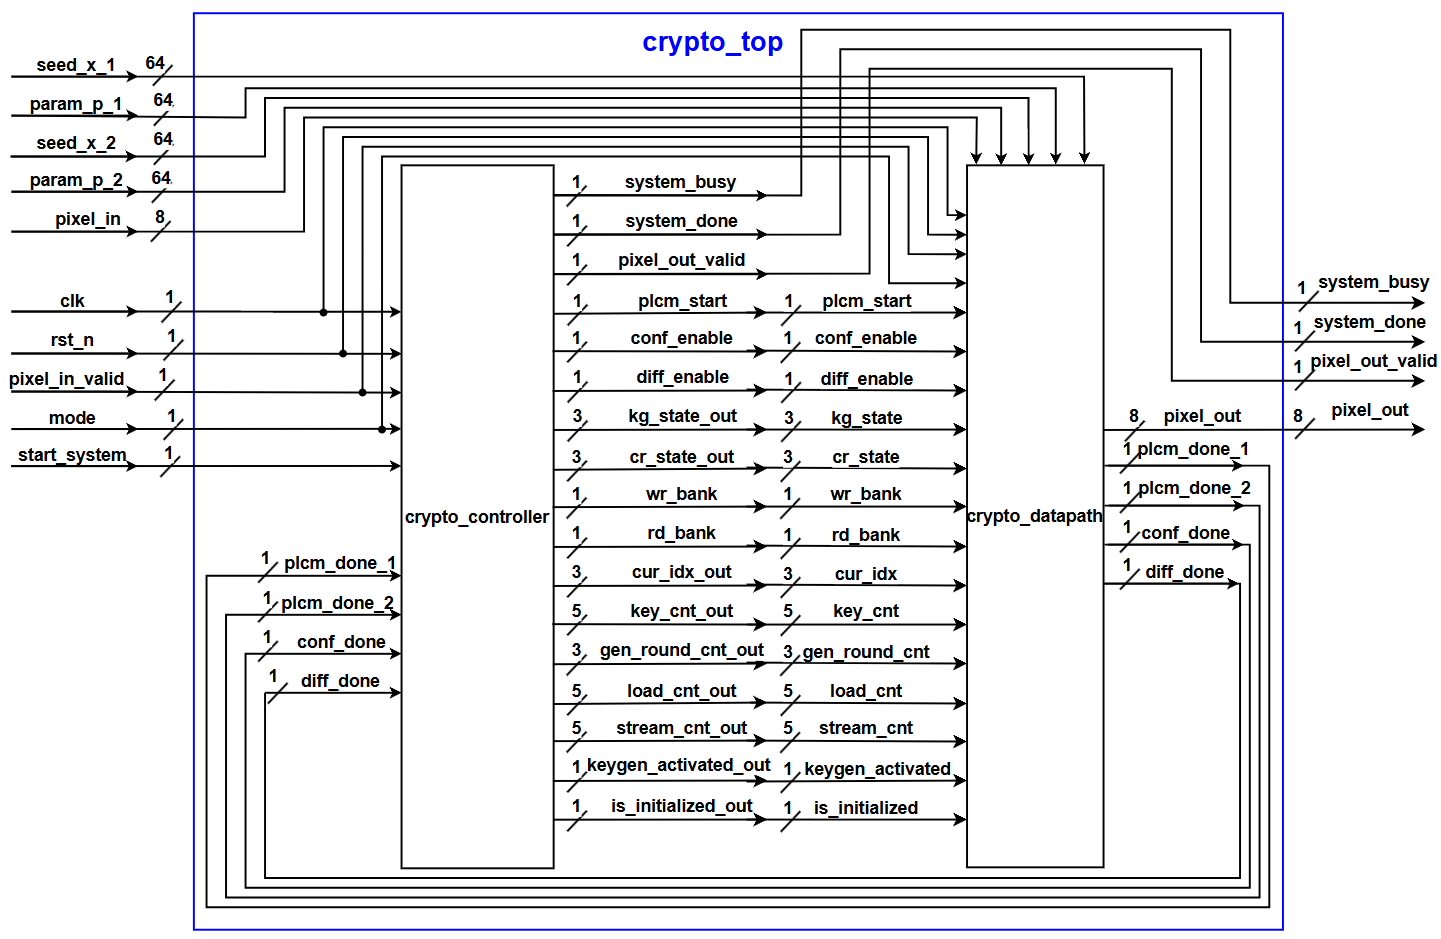
\includegraphics[width=1\textwidth]{Figures/sdkht.png} % Ghi chú: Chèn hình Visio tổng quát gồm top, controller và datapath vào đây
	\caption{Sơ đồ khối kết nối nội bộ cấp hệ thống}
	\label{fig:crypto_top_sd}
\end{figure}

\textbf{Tổng quan tín hiệu vào/ra}

\begin{longtable}{|c|c|c|c|c|p{5cm}|}
	\caption{Bảng mô tả các tín hiệu ngõ vào/ra của vỏ bọc IP crypto\_top}
	\label{bang_crypto_top} \\
	\hline
	\textbf{Tín hiệu} & \textbf{Số bit} & \textbf{I/O} & \textbf{Reg/Wire} & \textbf{Mức hoạt động} & \textbf{Chức năng} \\ \hline
	\endfirsthead
	
	% --- Tiêu đề lặp lại ở đầu trang tiếp theo ---
	\hline
	\textbf{Tín hiệu} & \textbf{Số bit} & \textbf{I/O} & \textbf{Reg/Wire} & \textbf{Mức hoạt động} & \textbf{Chức năng} \\ \hline
	\endhead
	
	% --- Dòng chốt khi bảng kết thúc hoàn toàn ---
	\hline
	\endlastfoot
	
	% --- NỘI DUNG BẢNG ---
	clk              & 1  & I & Wire & Sườn lên  & Nguồn xung nhịp hệ thống chủ đạo. \\ \hline
	rst\_n           & 1  & I & Wire & Mức thấp  & Đặt lại toàn bộ lõi IP về trạng thái gốc. \\ \hline
	start\_system    & 1  & I & Wire & Mức cao   & Tín hiệu kích hoạt hệ thống bắt đầu nạp. \\ \hline
	mode             & 1  & I & Wire & N/A       & \texttt{0}: Mã hóa tiến, \texttt{1}: Giải mã lùi. \\ \hline
	seed\_x\_1       & 64 & I & Wire & N/A       & Mầm khởi tạo $u_0$ cho lõi PLCM số 1. \\ \hline
	param\_p\_1      & 64 & I & Wire & N/A       & Tham số hệ thống $p$ cho lõi PLCM số 1. \\ \hline
	seed\_x\_2       & 64 & I & Wire & N/A       & Mầm khởi tạo $u_0$ cho lõi PLCM số 2. \\ \hline
	param\_p\_2      & 64 & I & Wire & N/A       & Tham số hệ thống $p$ cho lõi PLCM số 2. \\ \hline
	pixel\_in        & 8  & I & Wire & N/A       & Chuỗi dữ liệu 8-bit đầu vào (Bản rõ/Bản mã). \\ \hline
	pixel\_in\_valid & 1  & I & Wire & Mức cao   & Cờ xác nhận byte ngõ vào đang hợp lệ. \\ \hline
	system\_busy     & 1  & O & Wire & Mức cao   & Báo hiệu hệ thống tạm ngưng nhận dữ liệu. \\ \hline
	system\_done     & 1  & O & Wire & Mức cao   & Báo hiệu hoàn tất luồng xử lý 25 bytes. \\ \hline
	pixel\_out       & 8  & O & Wire & N/A       & Chuỗi dữ liệu 8-bit đầu ra (Bản mã/Bản rõ). \\ \hline
	pixel\_out\_valid& 1  & O & Wire & Mức cao   & Cờ xác nhận byte ngõ ra đang hợp lệ. \\ 
\end{longtable}


\subsubsection{Khối crypto\_controller}
\textbf{Đặc tả chức năng hoạt động}

Khối \texttt{crypto\_controller} đảm nhận vai trò trung tâm điều khiển trong kiến trúc của hệ thống mật mã. Chức năng cốt lõi của khối là điều phối toàn bộ chu trình xử lý dữ liệu và định thời thông qua việc xuất các tín hiệu mệnh lệnh, địa chỉ truy xuất bộ nhớ và các cờ trạng thái. Để giảm thiểu tối đa diện tích silicon và tài nguyên thanh ghi trên vi mạch, khối này được tối ưu hóa theo hướng thuần logic điều khiển, hoàn toàn không chứa các mạch toán học phức tạp hay các mảng bộ nhớ RAM.

Hệ thống ứng dụng kiến trúc đa luồng bất đồng bộ với hai máy trạng thái chạy song song: máy sinh khóa và máy điều phối mật mã. Sự phân tách này giúp giảm bớt số lượng trạng thái cần giải mã của mạch tổ hợp, đồng thời cho phép hệ thống che khuất độ trễ bằng cách vừa tính toán luồng khóa mới, vừa xử lý chuỗi hệ số DC cùng một lúc. Hai máy trạng thái này giao tiếp với nhau theo cơ chế bắt tay thông qua cờ báo trạng thái của bộ đệm khóa. Trong quá trình vận hành, hệ thống liên tục tính toán và xuất các bộ đếm vòng lặp, biến trạng thái (\texttt{kg\_state}, \texttt{cr\_state}) cũng như chỉ số phân vùng RAM để cấu hình mạng lưới bộ ghép kênh, từ đó định hướng chính xác luồng dữ liệu tuần tự đi qua các khối toán học.

\textbf{Trạng thái hoạt động}

Hoạt động của khối tuân theo sự điều phối nhịp nhàng của hai chu trình máy trạng thái độc lập. Trình tự vận hành bắt đầu với máy sinh khóa, khi nó xuất tín hiệu \texttt{plcm\_start} điều khiển lõi hỗn loạn chạy không tải trong 100 chu kỳ đầu tiên nhằm triệt tiêu hoàn toàn hiệu ứng chuyển tiếp của thuật toán. Sau giai đoạn này, máy trạng thái tự động lặp lại quy trình trích xuất tham số hoán vị và sinh ra chuỗi 25 byte khóa giả ngẫu nhiên, lưu tạm vào mảng bộ nhớ trước khi nhận được yêu cầu truy xuất.

Song song với quá trình trên, máy điều phối mật mã sẽ được khởi tạo bằng việc nạp nối tiếp luồng 25 byte dữ liệu hệ số DC. Ngay sau khi xác nhận tín hiệu luồng khóa đã sẵn sàng, máy điều phối lần lượt phát các xung kích hoạt \texttt{conf\_enable} và \texttt{diff\_enable} cho các cấu trúc đường ống xáo trộn và khuếch tán. Tùy thuộc vào trạng thái tín hiệu \texttt{mode}, trình tự thực thi của hai khối này sẽ được đảo ngược cho phù hợp. Quá trình xử lý chéo này được lặp lại chính xác 5 vòng trước khi hệ thống kích hoạt lệnh xuất chuỗi dữ liệu thành phẩm ra bên ngoài.

\textbf{Sơ đồ chân I/O}

\begin{figure}[H]
	\centering
	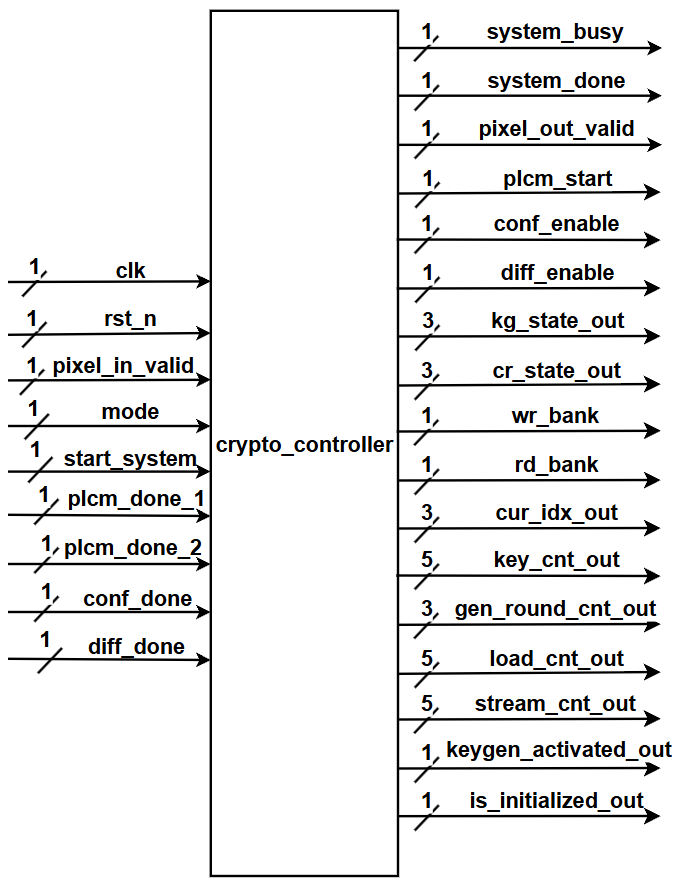
\includegraphics[width=0.5\textwidth]{Figures/control_io.png}
	\caption{Sơ đồ chân I/O khối crypto\_controller}
	\label{fig:control_io}
\end{figure}

\textbf{Tổng quan tín hiệu vào/ra}

\begin{table}[H]
	\centering
	\caption{Bảng mô tả tín hiệu ngõ vào/ra của khối crypto\_controller}
	\begin{tabular}{|c|c|c|c|c|p{4cm}|}
		\hline
		\textbf{Tín hiệu} & \textbf{Số bit} & \textbf{I/O} & \textbf{Reg/Wire} & \textbf{Mức hoạt động} & \textbf{Chức năng} \\ \hline
		clk / rst\_n     & 1 & I & Wire & N/A      & Nguồn xung nhịp và Reset hệ thống. \\ \hline
		start\_system    & 1 & I & Wire & Mức cao  & Tín hiệu kích hoạt từ thiết bị ngoại vi. \\ \hline
		mode             & 1 & I & Wire & N/A      & \texttt{0}: Mã hóa, \texttt{1}: Giải mã. \\ \hline
		plcm/conf/diff\_done& 1 & I & Wire & Mức cao & Cờ phản hồi hoàn tất từ module toán học. \\ \hline
		plcm\_start      & 1 & O & Reg  & Mức cao  & Xung kích hoạt hoạt động của lõi hỗn loạn. \\ \hline
		conf/diff\_enable& 1 & O & Reg  & Mức cao  & Xung kích hoạt các đường ống tổ hợp. \\ \hline
		kg/cr\_state\_out& 3 & O & Wire & N/A      & Biến trạng thái gửi sang cấu hình bộ ghép kênh. \\ \hline
		load/stream\_cnt & 5 & O & Wire & N/A      & Địa chỉ truy xuất RAM ($0 \rightarrow 24$). \\ \hline
	\end{tabular}
	\label{bang_crypto_controller}
\end{table}

\textbf{Lưu đồ thuật toán }

\begin{figure}[H]
	\centering
	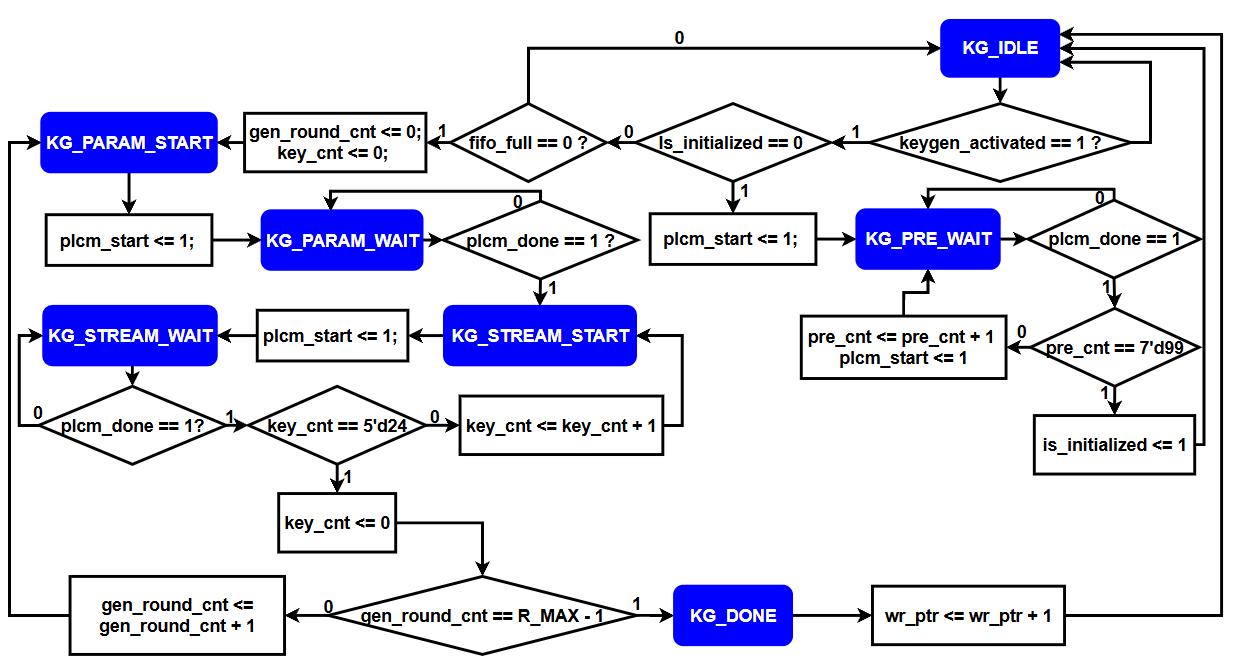
\includegraphics[width=1\textwidth]{Figures/key_ld.png}
	\caption{Lưu đồ thuật toán FSM sinh khoá của crypto\_controller}
	\label{fig:key_ld}
\end{figure}

\begin{figure}[H]
	\centering
	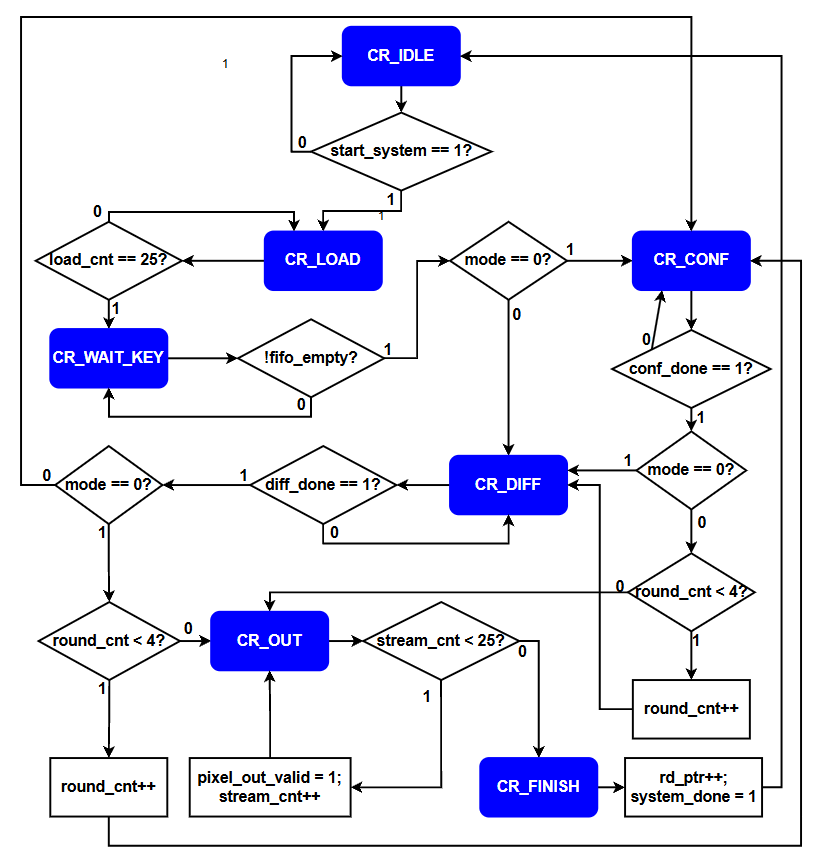
\includegraphics[width=0.8\textwidth]{Figures/fsm_crypt.png}
	\caption{Lưu đồ thuật toán FSM Máy điều phối Mật mã}
	\label{fig:fsm_crypt}
\end{figure}

\textbf{Timing diagram}

\begin{figure}[H]
	\centering
	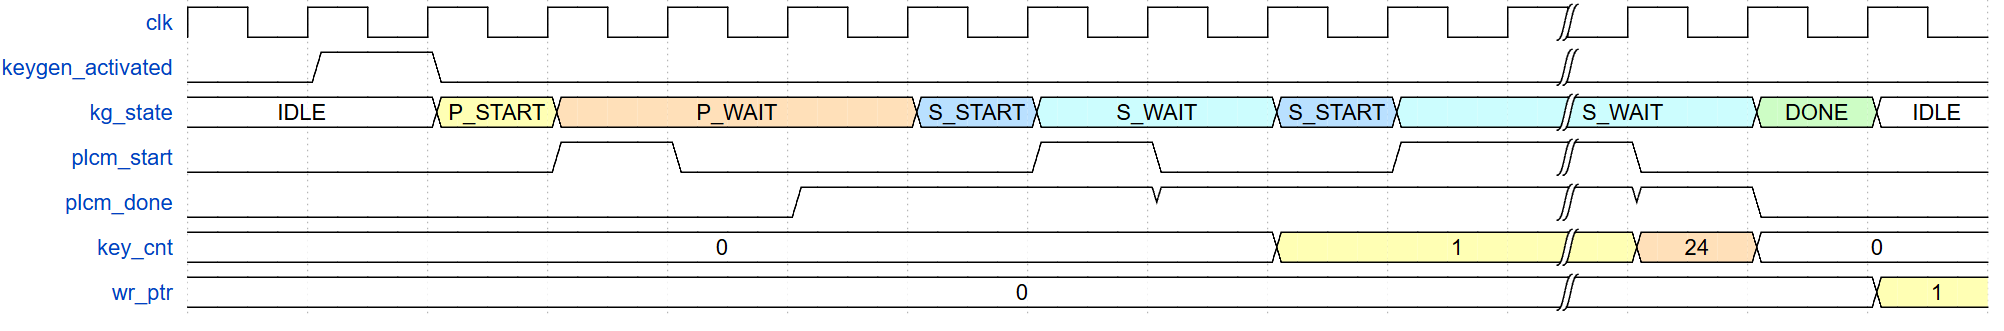
\includegraphics[width=1\textwidth]{Figures/key_td.png}
	\caption{Timing diagram Khối sinh khoá}
	\label{fig:key_td}
\end{figure}

\begin{figure}[H]
	\centering
	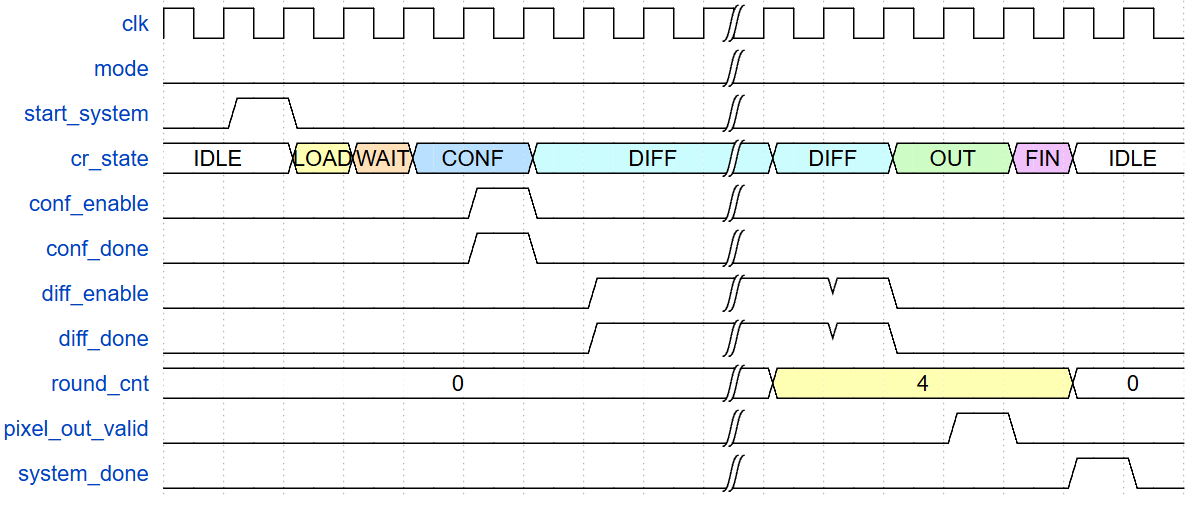
\includegraphics[width=1\textwidth]{Figures/cryp_td.png}
	\caption{Timing diagram Khối mật mã}
	\label{fig:cryp_td}
\end{figure}


\subsubsection{Khối crypto\_datapath}
\textbf{Đặc tả chức năng hoạt động}

Đối lập với phân hệ điều khiển, khối \texttt{crypto\_datapath} đảm nhận vai trò đường dẫn dữ liệu của toàn bộ hệ thống. Đây là một khối thuần cấu trúc, bao gồm mạng lưới mạch tổ hợp và các vùng nhớ nội bộ, hoàn toàn không chứa máy trạng thái. Nhiệm vụ trọng tâm của khối là tiếp nhận các luồng dữ liệu lớn từ ngoại vi, lưu trữ an toàn vào bộ nhớ ngầm và trực tiếp thực thi các phép toán ma trận phức tạp dựa trên mệnh lệnh định tuyến từ phân hệ điều khiển.

Đường dẫn dữ liệu được thiết kế theo cấu trúc hướng bộ nhớ, sở hữu ba mảng RAM nội bộ cực kỳ quan trọng: bộ nhớ \texttt{data\_ram} chứa dữ liệu gốc hoặc thành phẩm, bộ đệm \texttt{temp\_ram} dùng để hoán chuyển trạng thái giữa các vòng lặp, và bộ nhớ \texttt{ks\_ram} chứa luồng khóa giả ngẫu nhiên. Phân hệ này tích hợp và cung cấp đường dẫn dữ liệu trực tiếp cho bốn lõi toán học ở cấp độ thanh ghi, bao gồm hai lõi sinh khóa \texttt{plcm}, một khối xáo trộn \texttt{confusion} và một khối khuếch tán \texttt{diffusion}.

\textbf{Kiến trúc nội bộ khối crypto\_datapath}

Điểm sáng trong kiến trúc nội bộ của khối là các luồng dữ liệu không được kết nối vật lý cố định theo dạng nối tiếp. Thay vào đó, toàn bộ dữ liệu xuất ra từ các mảng RAM hay kết quả tính toán từ các lõi hỗn loạn đều hội tụ tại một trạm điều phối trung tâm bao gồm mạng lưới các bộ ghép kênh (MUX).

Trạm định tuyến này chịu sự điều khiển trực tiếp từ các biến trạng thái \texttt{cr\_state}, \texttt{kg\_state} và cờ cấu hình luồng \texttt{mode} do khối \texttt{crypto\_controller} cấp xuống. Tùy thuộc vào chu kỳ vận hành hiện tại, hệ thống tổ hợp sẽ tự động bẻ ghi để quyết định khối toán học nào được phép ghi dữ liệu vào RAM, và mảng RAM nào sẽ xuất dữ liệu ra cho khối tính toán đọc. Nhờ cơ chế kiến trúc linh hoạt này, các khối \texttt{confusion} và \texttt{diffusion} có thể dễ dàng chia sẻ và tái sử dụng chung các mảng RAM một cách liên tục trong suốt 5 vòng lặp mã hóa hoặc giải mã mà không bao giờ gây ra hiện tượng xung đột trên đường truyền dữ liệu.

\begin{figure}[H]
	\centering
	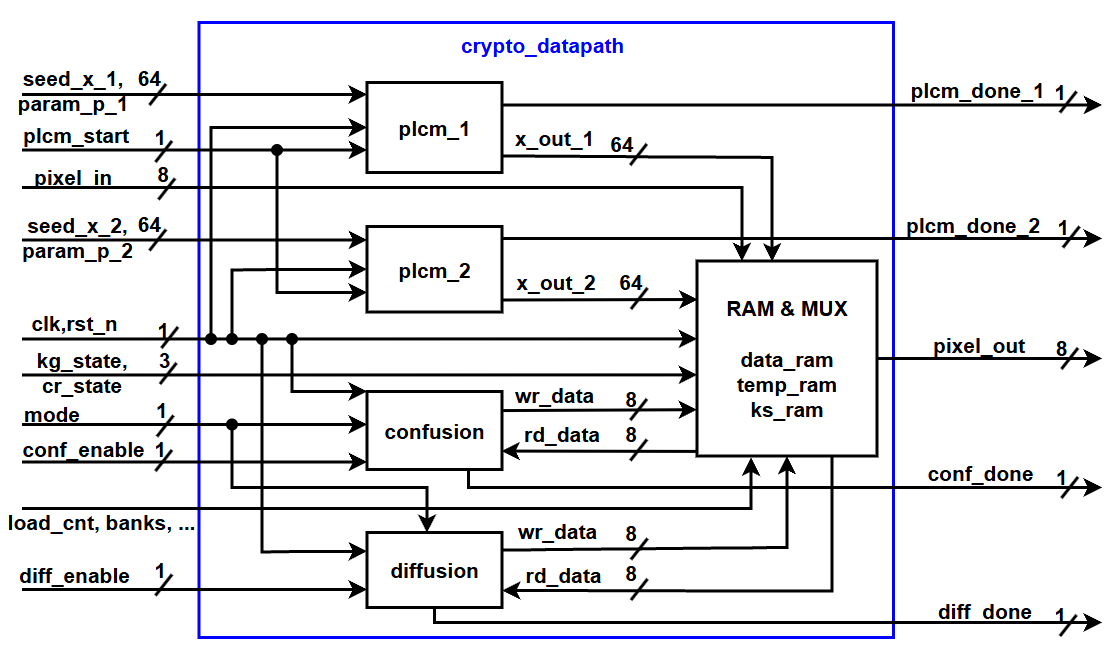
\includegraphics[width=0.9\textwidth]{Figures/datapath_sd.png} 
	\caption{Sơ đồ kiến trúc nội bộ khối crypto\_datapath}
	\label{fig:datapath_sd}
\end{figure}

\textbf{Sơ đồ chân I/O}

\begin{figure}[H]
	\centering
	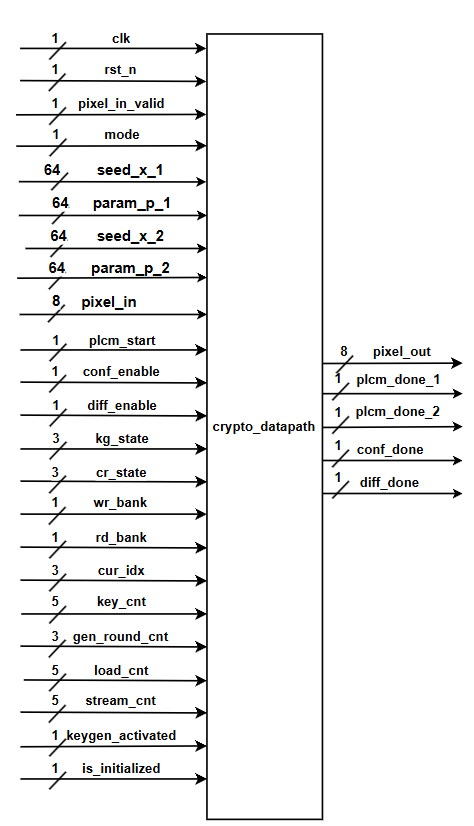
\includegraphics[width=0.4\textwidth]{Figures/datapath_io.png}
	\caption{Sơ đồ chân I/O khối crypto\_datapath}
	\label{fig:datapath_io}
\end{figure}

\textbf{Tổng quan tín hiệu vào/ra}

Do bản chất là một hệ thống định tuyến và xử lý thụ động, cấu trúc tín hiệu giao tiếp của đường dẫn dữ liệu chủ yếu bao gồm các kênh nạp dữ liệu từ thiết bị ngoại vi và các ngõ nhận lệnh điều khiển trực tiếp từ máy trạng thái trung tâm.

\begin{longtable}{|c|c|c|c|c|p{4cm}|}
	\caption{Bảng mô tả tín hiệu ngõ vào/ra của khối crypto\_datapath}
	\label{bang_crypto_datapath} \\
	\hline
	\textbf{Tín hiệu} & \textbf{Số bit} & \textbf{I/O} & \textbf{Reg/Wire} & \textbf{Mức hoạt động} & \textbf{Chức năng} \\ \hline
	\endfirsthead
	
	% --- Tiêu đề lặp lại ở trang mới (không có dòng chữ chú thích) ---
	\hline
	\textbf{Tín hiệu} & \textbf{Số bit} & \textbf{I/O} & \textbf{Reg/Wire} & \textbf{Mức hoạt động} & \textbf{Chức năng} \\ \hline
	\endhead
	
	% --- NỘI DUNG BẢNG ---
	clk / rst\_n      & 1  & I & Wire & N/A      & Nguồn xung nhịp và Reset thanh ghi đường ống. \\ \hline
	seed/param        & 64 & I & Wire & N/A      & Bus tín hiệu mầm tĩnh và tham số hệ thống. \\ \hline
	pixel\_in         & 8  & I & Wire & N/A      & Bus nhận chuỗi byte dữ liệu hệ số DC đầu vào. \\ \hline
	pixel\_out        & 8  & O & Reg  & N/A      & Bus xuất chuỗi byte dữ liệu sau khi xử lý. \\ \hline
	plcm\_start       & 1  & I & Wire & Mức cao  & Tín hiệu kích hoạt hoạt động lõi hỗn loạn. \\ \hline
	conf/diff\_enable & 1  & I & Wire & Mức cao  & Tín hiệu kích hoạt các đường ống dữ liệu. \\ \hline
	kg/cr\_state      & 3  & I & Wire & N/A      & Tín hiệu trạng thái FSM điều khiển mạng MUX. \\ \hline
	load/stream\_cnt  & 5  & I & Wire & N/A      & Địa chỉ truy xuất các mảng bộ nhớ RAM nội bộ. \\ \hline
	plcm/conf/diff\_done& 1 & O & Wire & Mức cao & Cờ trạng thái báo hiệu module hoàn tất xử lý. \\ \hline
\end{longtable}

%\subsection{Đặc tả chi tiết các khối con}
%
%\subsubsection{Khối crypto\_top}
%\textbf{Đặc tả chức năng hoạt động} 
%
%Khối \texttt{crypto\_top} đóng vai trò là lõi IP (Intellectual Property) mức cao nhất trong quy trình thiết kế phần cứng của toàn bộ hệ thống mật mã. Đặc điểm nổi bật nhất của khối này là nó được thiết kế theo dạng thuần cấu trúc (Structural Modeling) và mang tính chất thụ động. Khác với các module bên trong, bản thân \texttt{crypto\_top} hoàn toàn không chứa máy trạng thái hữu hạn (FSM) hay bất kỳ mạch tổ hợp tính toán độc lập nào. Thay vào đó, nó đóng vai trò là một lớp vỏ bọc (Wrapper) vững chắc nhằm bao bọc, định tuyến tín hiệu và kết nối hai phân hệ cốt lõi của hệ thống: khối điều khiển trung tâm \texttt{crypto\_controller} và khối đường dẫn dữ liệu \texttt{crypto\_datapath}.
%
%Nhiệm vụ trọng tâm của khối top là phân bổ các luồng tín hiệu giao tiếp ngoại vi một cách tối ưu và khoa học nhất. Cụ thể, đối với các tín hiệu mang tính chất điều khiển tiến trình như xung kích hoạt \texttt{start\_system} hay cờ xác nhận dữ liệu \texttt{pixel\_in\_valid}, mạch sẽ dẫn trực tiếp chúng vào khối \texttt{crypto\_controller} để đồng bộ hóa hoạt động của các máy trạng thái bên trong. Ngược lại, đối với các bus dữ liệu có kích thước lớn, bao gồm các vector tham số mầm \texttt{seed\_x}, thông số không gian \texttt{param\_p} và chuỗi điểm ảnh đầu vào \texttt{pixel\_in}, hệ thống sẽ kết nối thẳng đến khối \texttt{crypto\_datapath} để ghi trực tiếp vào các mảng RAM nội bộ. Việc bóc tách đường truyền này giúp tối ưu hóa định tuyến vật lý, giảm thiểu độ trễ trên đường dẫn và giảm tải khối lượng công việc đáng kể cho phân hệ điều khiển.
%
%Ở chiều phản hồi, các cờ báo hiệu tiến độ hoàn thành từ phân hệ xử lý dữ liệu, chẳng hạn như \texttt{plcm\_done}, \texttt{conf\_done}, và \texttt{diff\_done}, sẽ được mạch vòng ngược trở lại ngõ vào của phân hệ điều khiển để làm điều kiện chuyển đổi trạng thái (State Transition). Sự phối hợp nhịp nhàng, logic giữa các luồng tín hiệu song song này đã tạo nên một kiến trúc máy trạng thái kết hợp đường dẫn dữ liệu (FSMD) khép kín, đảm bảo hệ thống hoạt động đồng bộ, an toàn và tối ưu hóa tối đa lượng tài nguyên phần cứng tiêu thụ trên vi mạch.
%
%\textbf{Các tín hiệu vào/ra}
%
%Giao diện của lõi IP được quy hoạch một cách nghiêm ngặt theo các tiêu chuẩn thiết kế vi mạch chung nhằm đảm bảo khả năng tích hợp linh hoạt, dễ dàng ghép nối với các vi điều khiển hoặc các hệ thống trên chip (SoC) bên ngoài. Cụ thể, các tín hiệu giao tiếp được chia thành các nhóm chức năng độc lập. Nhóm xung nhịp và đặt lại hệ thống bao gồm tín hiệu đồng hồ \texttt{clk} và tín hiệu reset bất đồng bộ tích cực mức thấp \texttt{rst\_n}. Nhóm điều khiển bao gồm lệnh kích hoạt hệ thống \texttt{start\_system} và cờ \texttt{mode} dùng để thiết lập cấu hình hoạt động là mã hóa tiến hay giải mã lùi. Nhóm thông số mật mã đóng vai trò tiếp nhận các vector 64-bit nhằm cung cấp tham số hình học và mầm khởi tạo cho hai module hỗn loạn bên trong. Đối với luồng dữ liệu, hệ thống cung cấp các kênh truyền nhận tuần tự 8-bit (\texttt{pixel\_in} và \texttt{pixel\_out}) đi kèm với các cờ xác nhận tính hợp lệ tương ứng. Cuối cùng, nhóm cờ trạng thái ngoại vi cung cấp các tín hiệu \texttt{system\_busy} và \texttt{system\_done} để thiết bị ngoại vi có thể giám sát theo thời gian thực toàn bộ chu trình xử lý của lõi mật mã.
%
%\textbf{Sơ đồ khối}
%
%\begin{figure}[H]
%	\centering
%	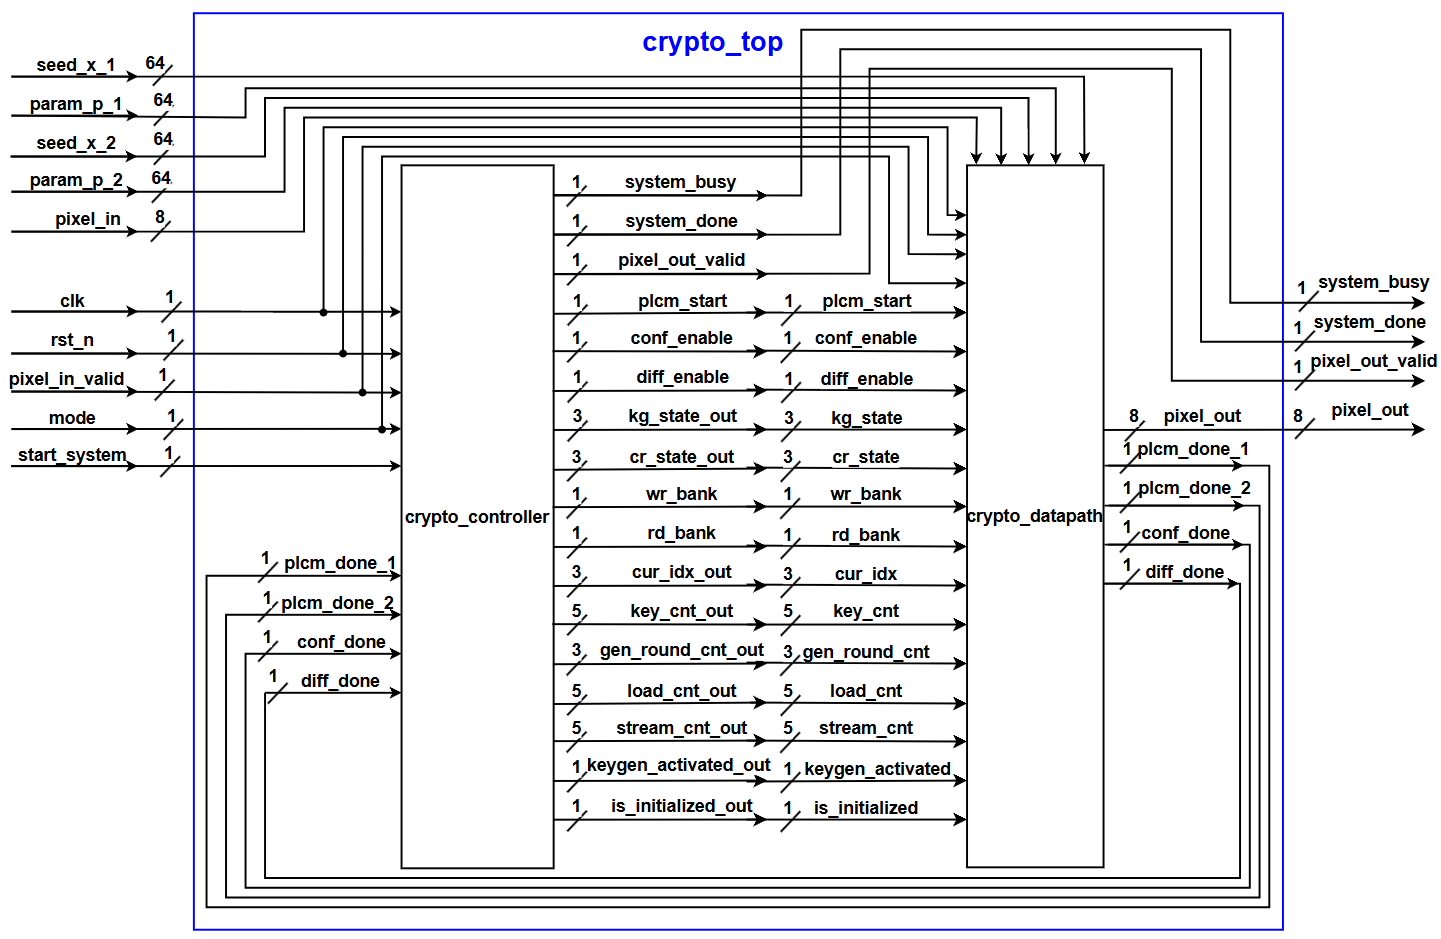
\includegraphics[width=1\textwidth]{Figures/sdkht.png} 
%	\caption{Sơ đồ khối kết nối nội bộ cấp hệ thống (crypto\_top)}
%	\label{fig:crypto_top_sd}
%\end{figure}
%
%\textbf{Tổng quan tín hiệu vào/ra}
%
%\begin{longtable}{|c|c|c|c|c|p{5.5cm}|}
%	\caption{Bảng mô tả các tín hiệu ngõ vào/ra của vỏ bọc IP crypto\_top}
%	\label{bang_crypto_top} \\
%	\hline
%	\textbf{Tín hiệu} & \textbf{Số bit} & \textbf{I/O} & \textbf{Reg/Wire} & \textbf{Mức hoạt động} & \textbf{Chức năng} \\ \hline
%	\endfirsthead
%	
%	\hline
%	\textbf{Tín hiệu} & \textbf{Số bit} & \textbf{I/O} & \textbf{Reg/Wire} & \textbf{Mức hoạt động} & \textbf{Chức năng} \\ \hline
%	\endhead
%	
%	\hline
%	\endlastfoot
%	
%	clk              & 1  & I & Wire & Sườn lên  & Nguồn xung nhịp hệ thống chủ đạo. \\ \hline
%	rst\_n           & 1  & I & Wire & Mức thấp  & Đặt lại toàn bộ lõi IP về trạng thái gốc. \\ \hline
%	start\_system    & 1  & I & Wire & Mức cao   & Tín hiệu kích hoạt hệ thống bắt đầu nạp. \\ \hline
%	mode             & 1  & I & Wire & N/A       & \texttt{0}: Mã hóa tiến, \texttt{1}: Giải mã lùi. \\ \hline
%	seed\_x\_1       & 64 & I & Wire & N/A       & Mầm khởi tạo cho lõi sinh khóa thứ 1. \\ \hline
%	param\_p\_1      & 64 & I & Wire & N/A       & Tham số hệ thống cho lõi sinh khóa thứ 1. \\ \hline
%	seed\_x\_2       & 64 & I & Wire & N/A       & Mầm khởi tạo cho lõi sinh khóa thứ 2. \\ \hline
%	param\_p\_2      & 64 & I & Wire & N/A       & Tham số hệ thống cho lõi sinh khóa thứ 2. \\ \hline
%	pixel\_in        & 8  & I & Wire & N/A       & Chuỗi dữ liệu 8-bit đầu vào (Bản rõ/Bản mã). \\ \hline
%	pixel\_in\_valid & 1  & I & Wire & Mức cao   & Cờ xác nhận byte ngõ vào đang hợp lệ. \\ \hline
%	system\_busy     & 1  & O & Wire & Mức cao   & Báo hiệu hệ thống tạm ngưng nhận dữ liệu. \\ \hline
%	system\_done     & 1  & O & Wire & Mức cao   & Báo hiệu hoàn tất luồng xử lý 25 bytes. \\ \hline
%	pixel\_out       & 8  & O & Wire & N/A       & Chuỗi dữ liệu 8-bit đầu ra (Bản mã/Bản rõ). \\ \hline
%	pixel\_out\_valid& 1  & O & Wire & Mức cao   & Cờ xác nhận byte ngõ ra đang hợp lệ. \\ 
%\end{longtable}
%
%
%\subsubsection{Khối crypto\_controller}
%\textbf{Đặc tả chức năng hoạt động}
%
%Khối \texttt{crypto\_controller} đảm nhận vai trò trung tâm não bộ, điều khiển toàn bộ luồng thực thi trong kiến trúc FSMD của hệ thống mật mã. Chức năng cốt lõi của khối này là giám sát, định thời và điều phối toàn bộ chu trình xử lý dữ liệu thông qua việc phát ra các tín hiệu mệnh lệnh kích hoạt, cung cấp địa chỉ truy xuất bộ nhớ chính xác và cập nhật các cờ trạng thái liên tục. Với định hướng thiết kế nhằm tiết kiệm tối đa diện tích silicon và tài nguyên thanh ghi khi triển khai trên vi mạch thực tế, khối này được xây dựng theo hướng thuần logic điều khiển. Nó hoàn toàn không chứa bất kỳ một phép toán số học phức tạp hay mảng bộ nhớ lưu trữ nào, nhường toàn bộ gánh nặng này cho phân hệ dữ liệu.
%
%Điểm đột phá về mặt kiến trúc của khối điều khiển là việc ứng dụng mô hình đa luồng bất đồng bộ, trong đó hệ thống sử dụng hai máy trạng thái hữu hạn (FSM) chạy song song: một máy chuyên trách việc sinh khóa và một máy điều phối tiến trình mật mã trung tâm. Sự phân tách này không chỉ giúp giảm bớt sự phình to của số lượng trạng thái cần giải mã trong mạch tổ hợp, mà còn cho phép hệ thống áp dụng kỹ thuật che khuất độ trễ (Latency Hiding). Nhờ đó, hệ thống có thể vừa tận dụng thời gian trống để tính toán ra luồng khóa mới, vừa song song tiến hành xử lý chuỗi hệ số DC, tối đa hóa thông lượng đầu ra. Hai máy trạng thái độc lập này được thiết kế để giao tiếp với nhau theo cơ chế bắt tay (Handshake) thông qua cờ báo trạng thái của bộ đệm khóa. Trong suốt quá trình vận hành, hệ thống FSM sẽ liên tục xuất ra các biến trạng thái quan trọng như \texttt{kg\_state} và \texttt{cr\_state} cùng các bộ đếm địa chỉ để cấu hình mạng lưới bộ ghép kênh, qua đó thiết lập chính xác lộ trình cho chuỗi dữ liệu đi qua các cỗ máy toán học một cách an toàn.
%
%\textbf{Trạng thái hoạt động}
%
%Quy trình vận hành của hệ thống phụ thuộc vào sự phối hợp nhịp nhàng của hai chu trình máy trạng thái độc lập. Trình tự bắt đầu với máy trạng thái sinh khóa, khi hệ thống vừa được cấp nguồn, nó sẽ xuất tín hiệu \texttt{plcm\_start} để ép lõi hỗn loạn chạy không tải trong 100 chu kỳ xung nhịp đầu tiên. Bước tiền khởi tạo (Pre-iteration) này cực kỳ quan trọng trong mật mã học hỗn loạn nhằm triệt tiêu hoàn toàn hiệu ứng quá độ và đảm bảo chuỗi ngõ ra đạt được đặc tính thống kê ngẫu nhiên tốt nhất. Sau khi kết thúc giai đoạn này, máy trạng thái tự động lặp lại quy trình trích xuất tham số không gian và sinh ra chuỗi 25 byte khóa giả ngẫu nhiên, lưu trữ toàn bộ vào mảng bộ nhớ tạm thời trước khi máy điều phối mật mã gửi yêu cầu truy xuất.
%
%Song song với quá trình tạo khóa, máy trạng thái điều phối mật mã sẽ bắt đầu chu trình của mình bằng việc tiếp nhận lệnh \texttt{start\_system} và nạp nối tiếp luồng 25 byte hệ số DC vào bộ đệm. Ngay khi xác nhận được cờ báo hiệu luồng khóa đã chuẩn bị sẵn sàng, máy điều phối lần lượt phát các xung kích hoạt \texttt{conf\_enable} và \texttt{diff\_enable} cho các cấu trúc đường ống xáo trộn và khuếch tán. Tùy thuộc vào trạng thái của tín hiệu \texttt{mode}, trình tự thực thi của hai khối này sẽ được đảo ngược để phù hợp với quy trình mã hóa tiến hoặc giải mã lùi. Quá trình luân chuyển dữ liệu qua lại giữa hai phân hệ toán học này được hệ thống giám sát và lặp lại chính xác 5 vòng để đảm bảo tính an toàn mật mã trước khi kích hoạt cờ \texttt{system\_done} để xuất toàn bộ chuỗi dữ liệu thành phẩm ra bên ngoài.
%
%\textbf{Sơ đồ chân I/O}
%
%\begin{figure}[H]
%	\centering
%	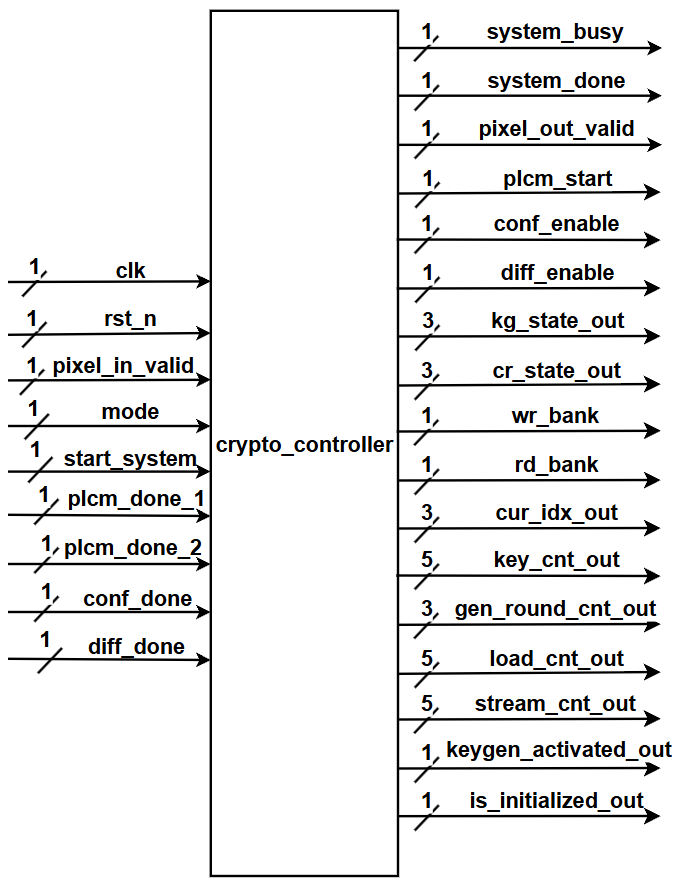
\includegraphics[width=0.6\textwidth]{Figures/control_io.png}
%	\caption{Sơ đồ chân I/O khối crypto\_controller}
%	\label{fig:control_io}
%\end{figure}
%
%\textbf{Tổng quan tín hiệu vào/ra}
%
%\begin{table}[H]
%	\centering
%	\caption{Bảng mô tả tín hiệu ngõ vào/ra của khối crypto\_controller}
%	\begin{tabular}{|c|c|c|c|c|p{5cm}|}
%		\hline
%		\textbf{Tín hiệu} & \textbf{Số bit} & \textbf{I/O} & \textbf{Reg/Wire} & \textbf{Mức hoạt động} & \textbf{Chức năng} \\ \hline
%		clk / rst\_n     & 1 & I & Wire & N/A      & Nguồn xung nhịp và Reset hệ thống. \\ \hline
%		start\_system    & 1 & I & Wire & Mức cao  & Tín hiệu kích hoạt từ thiết bị ngoại vi. \\ \hline
%		mode             & 1 & I & Wire & N/A      & \texttt{0}: Mã hóa, \texttt{1}: Giải mã. \\ \hline
%		plcm/conf/diff\_done& 1 & I & Wire & Mức cao & Cờ phản hồi hoàn tất từ module toán học. \\ \hline
%		plcm\_start      & 1 & O & Reg  & Mức cao  & Xung kích hoạt hoạt động của lõi hỗn loạn. \\ \hline
%		conf/diff\_enable& 1 & O & Reg  & Mức cao  & Xung kích hoạt các đường ống tổ hợp. \\ \hline
%		kg/cr\_state\_out& 3 & O & Wire & N/A      & Biến trạng thái gửi sang cấu hình bộ ghép kênh. \\ \hline
%		load/stream\_cnt & 5 & O & Wire & N/A      & Địa chỉ truy xuất RAM nội bộ ($0 \rightarrow 24$). \\ \hline
%	\end{tabular}
%	\label{bang_crypto_controller}
%\end{table}
%
%\textbf{Lưu đồ thuật toán }
%
%\begin{figure}[H]
%	\centering
%	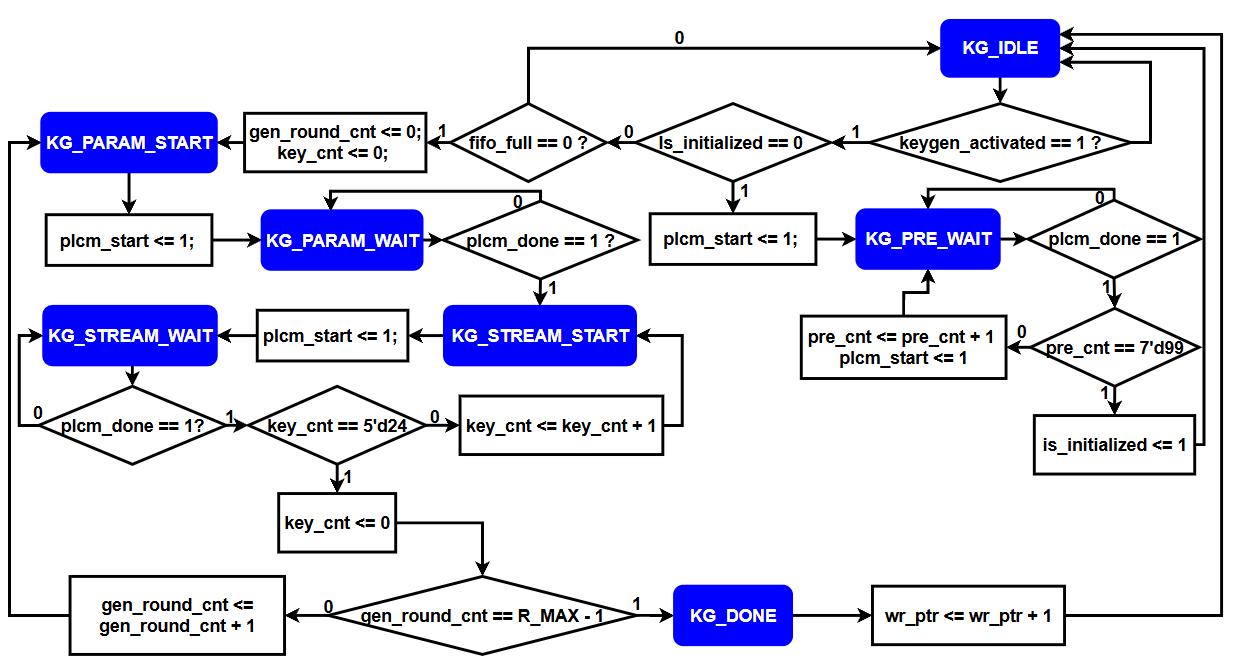
\includegraphics[width=1\textwidth]{Figures/key_ld.png}
%	\caption{Lưu đồ thuật toán FSM sinh khoá của crypto\_controller}
%	\label{fig:key_ld}
%\end{figure}
%
%\begin{figure}[H]
%	\centering
%	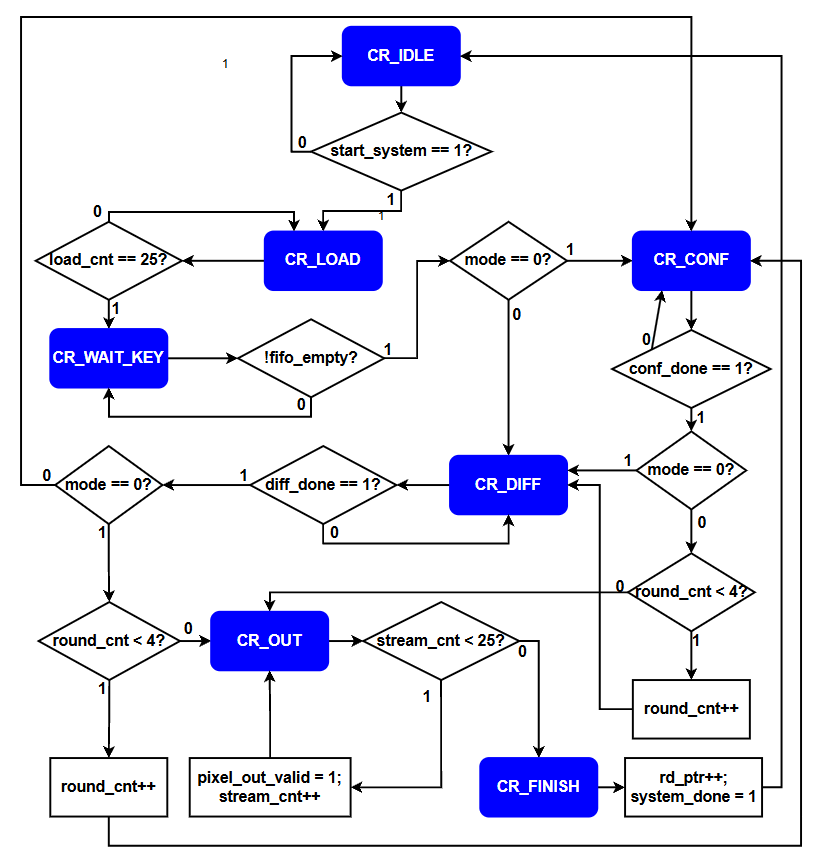
\includegraphics[width=1\textwidth]{Figures/fsm_crypt.png}
%	\caption{Lưu đồ thuật toán FSM Máy điều phối Mật mã}
%	\label{fig:fsm_crypt}
%\end{figure}
%
%\textbf{Giản đồ định thời}
%
%\begin{figure}[H]
%	\centering
%	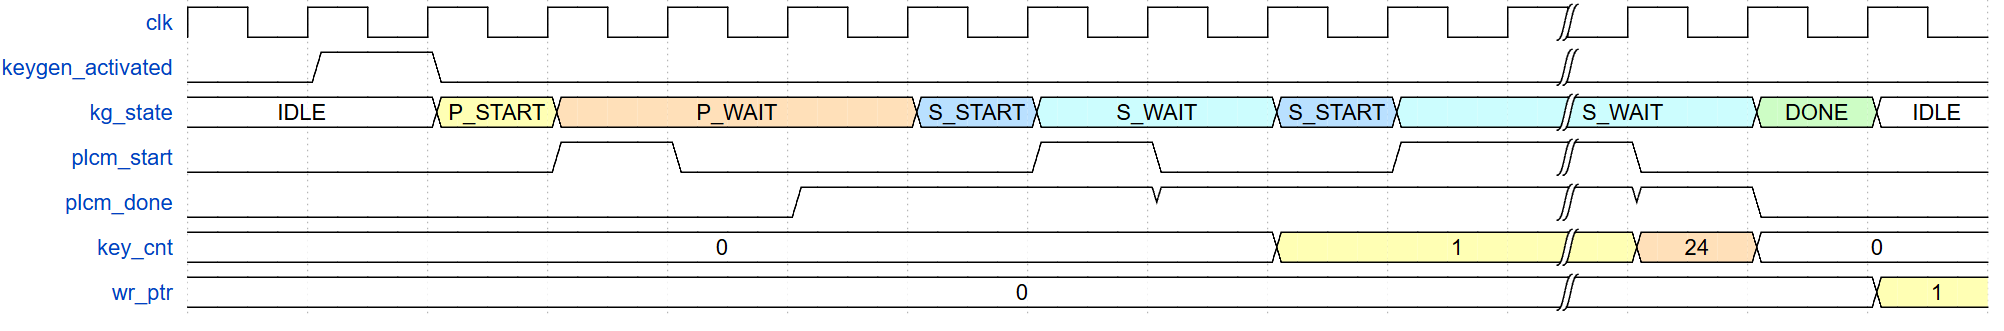
\includegraphics[width=1\textwidth]{Figures/key_td.png}
%	\caption{Giản đồ định thời Khối sinh khoá}
%	\label{fig:key_td}
%\end{figure}
%
%\begin{figure}[H]
%	\centering
%	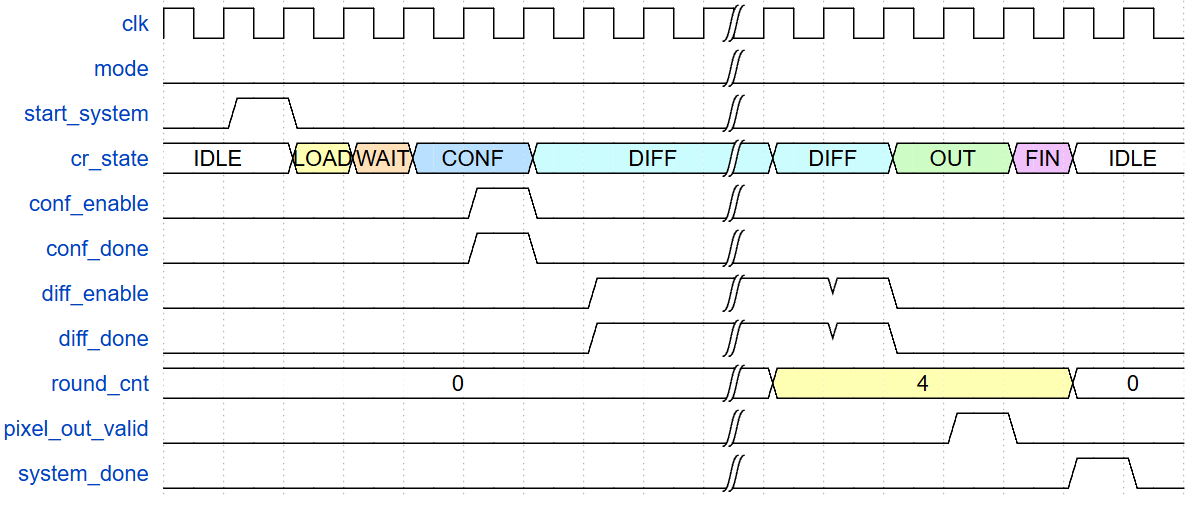
\includegraphics[width=1\textwidth]{Figures/cryp_td.png}
%	\caption{Giản đồ định thời Khối mật mã}
%	\label{fig:cryp_td}
%\end{figure}
%
%
%\subsubsection{Khối crypto\_datapath}
%\textbf{Đặc tả chức năng hoạt động}
%
%Nằm ở vị trí đối lập và phối hợp chặt chẽ với phân hệ điều khiển, khối \texttt{crypto\_datapath} đảm nhận toàn bộ vai trò định tuyến và tính toán cho đường dẫn dữ liệu của hệ thống. Khối này được thiết kế thuần cấu trúc, là nơi tập hợp toàn bộ mạng lưới mạch tổ hợp logic và các vùng nhớ bộ đệm nội bộ. Vì không chứa máy trạng thái điều khiển, khối này hoạt động hoàn toàn thụ động. Nhiệm vụ trọng tâm của nó là tiếp nhận các luồng dữ liệu kích thước lớn từ hệ thống ngoại vi, lưu trữ chúng một cách an toàn vào bộ nhớ ngầm, và thực thi các phép toán ma trận dày đặc dựa trên các mệnh lệnh kích hoạt từ khối điều khiển.
%
%Khối đường dẫn dữ liệu được thiết kế theo cấu trúc hướng bộ nhớ, sở hữu ba mảng RAM nội bộ cực kỳ quan trọng làm xương sống cho việc luân chuyển dữ liệu. Mảng thứ nhất là \texttt{data\_ram}, chịu trách nhiệm lưu trữ chuỗi dữ liệu gốc đầu vào hoặc dữ liệu thành phẩm chuẩn bị xuất ra. Mảng thứ hai là \texttt{temp\_ram}, đóng vai trò như một bộ đệm trung gian thiết yếu dùng để chứa dữ liệu hoán chuyển giữa các vòng lặp qua lại của thuật toán. Mảng thứ ba là \texttt{ks\_ram}, một vùng nhớ chuyên dụng chỉ để lưu trữ luồng khóa giả ngẫu nhiên phục vụ cho khâu khuếch tán. Bao quanh hệ thống bộ nhớ này, khối \texttt{crypto\_datapath} tích hợp và cung cấp đường truyền trực tiếp cho bốn cỗ máy toán học hoạt động ở cấp độ thanh ghi, bao gồm: hai lõi hỗn loạn sinh khóa \texttt{plcm}, một cấu trúc đường ống thực thi phép xáo trộn không gian \texttt{confusion}, và một đường ống chuyên trách phép khuếch tán giá trị \texttt{diffusion}.
%
%\textbf{Kiến trúc nội bộ khối crypto\_datapath}
%
%Điểm sáng đột phá trong kiến trúc nội bộ của khối là cơ chế định tuyến dữ liệu linh hoạt. Các luồng dữ liệu giữa các lõi toán học hoàn toàn không được kết nối vật lý cố định theo dạng tuyến tính thông thường. Thay vào đó, toàn bộ dữ liệu xuất ra từ các mảng RAM hay các kết quả vừa được tính toán xong từ các lõi hỗn loạn đều được hội tụ tại một trạm điều phối trung tâm. Trạm này được cấu thành từ một mạng lưới phức tạp các bộ ghép kênh (Multiplexer).
%
%Trạm định tuyến trung tâm này chịu sự giám sát và điều khiển trực tiếp từ các biến trạng thái \texttt{cr\_state}, \texttt{kg\_state} cùng cờ cấu hình luồng \texttt{mode} do máy trạng thái của khối điều khiển truyền xuống. Tùy thuộc vào việc hệ thống đang ở chu kỳ vận hành nào, mạng lưới bộ ghép kênh sẽ tự động bẻ ghi tín hiệu một cách nhịp nhàng. Nó sẽ quyết định lõi toán học nào được quyền ghi dữ liệu vào mảng RAM nào, đồng thời mảng RAM nào sẽ mở cổng để xuất dữ liệu ra cho khối tính toán tiếp nhận. Nhờ có cơ chế kiến trúc trung tâm qua bộ nhớ này, hệ thống đã tối ưu hóa được việc tái sử dụng phần cứng. Các khối \texttt{confusion} và \texttt{diffusion} có thể dễ dàng chia sẻ chung tài nguyên bộ nhớ một cách liên tục trong suốt 5 vòng lặp mã hóa hoặc giải mã mà tuyệt đối không bao giờ gây ra hiện tượng xung đột hay ghi đè dữ liệu trên đường truyền.
%
%\begin{figure}[H]
%	\centering
%	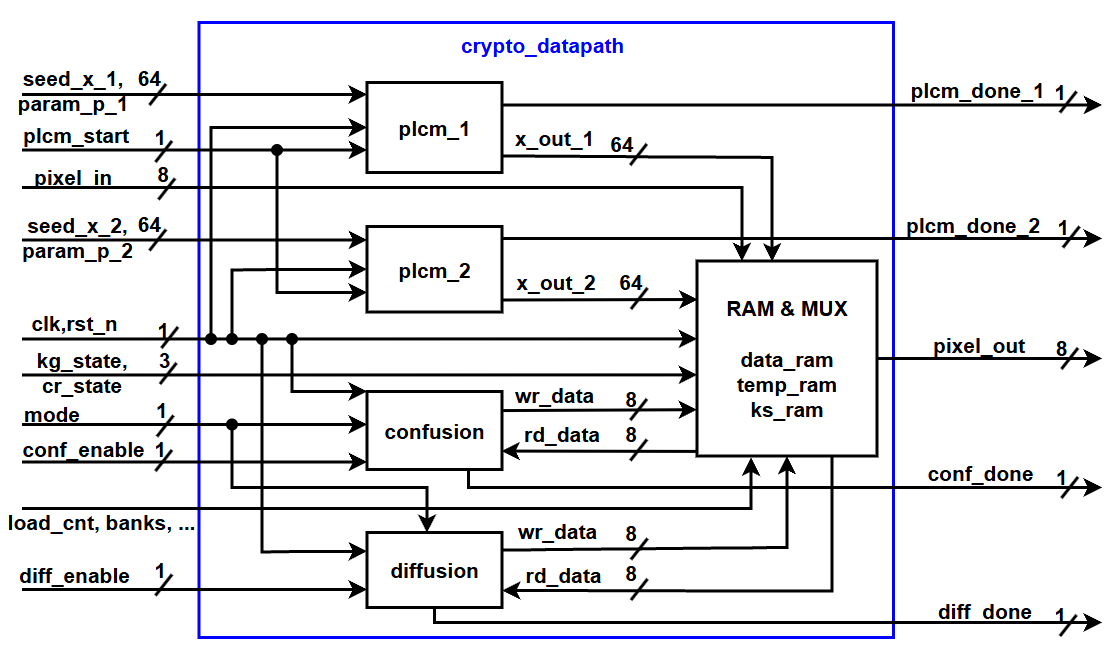
\includegraphics[width=0.9\textwidth]{Figures/datapath_sd.png} 
%	\caption{Sơ đồ kiến trúc nội bộ khối crypto\_datapath}
%	\label{fig:datapath_sd}
%\end{figure}
%
%\textbf{Sơ đồ chân I/O}
%
%\begin{figure}[H]
%	\centering
%	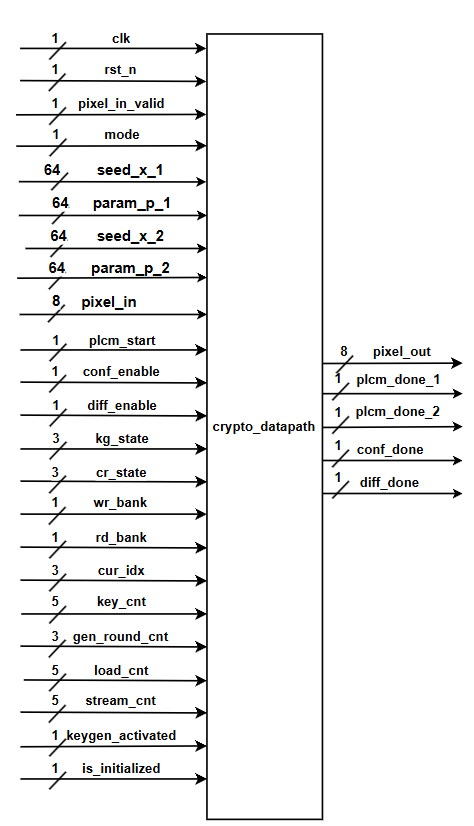
\includegraphics[width=0.5\textwidth]{Figures/datapath_io.png}
%	\caption{Sơ đồ chân I/O khối crypto\_datapath}
%	\label{fig:datapath_io}
%\end{figure}
%
%\textbf{Tổng quan tín hiệu vào/ra}
%
%Bản chất của khối đường dẫn dữ liệu là một hệ thống định tuyến và xử lý thụ động, do vậy, cấu trúc tín hiệu giao tiếp của nó chủ yếu tập trung vào việc nạp xuất dữ liệu từ các thiết bị ngoại vi và tiếp nhận các ngõ lệnh điều khiển trực tiếp từ máy trạng thái trung tâm để khởi chạy các module chức năng.
%
%\begin{longtable}{|c|c|c|c|c|p{5cm}|}
%	\caption{Bảng mô tả tín hiệu ngõ vào/ra của khối crypto\_datapath}
%	\label{bang_crypto_datapath} \\
%	\hline
%	\textbf{Tín hiệu} & \textbf{Số bit} & \textbf{I/O} & \textbf{Reg/Wire} & \textbf{Mức hoạt động} & \textbf{Chức năng} \\ \hline
%	\endfirsthead
%	
%	\hline
%	\textbf{Tín hiệu} & \textbf{Số bit} & \textbf{I/O} & \textbf{Reg/Wire} & \textbf{Mức hoạt động} & \textbf{Chức năng} \\ \hline
%	\endhead
%	
%	clk / rst\_n      & 1  & I & Wire & N/A      & Nguồn xung nhịp và Reset thanh ghi đường ống. \\ \hline
%	seed/param        & 64 & I & Wire & N/A      & Bus tín hiệu mầm tĩnh và tham số hệ thống. \\ \hline
%	pixel\_in         & 8  & I & Wire & N/A      & Bus nhận chuỗi byte dữ liệu hệ số DC đầu vào. \\ \hline
%	pixel\_out        & 8  & O & Reg  & N/A      & Bus xuất chuỗi byte dữ liệu sau khi xử lý. \\ \hline
%	plcm\_start       & 1  & I & Wire & Mức cao  & Tín hiệu kích hoạt hoạt động lõi hỗn loạn. \\ \hline
%	conf/diff\_enable & 1  & I & Wire & Mức cao  & Tín hiệu kích hoạt các đường ống dữ liệu. \\ \hline
%	kg/cr\_state      & 3  & I & Wire & N/A      & Tín hiệu trạng thái FSM điều khiển mạng MUX. \\ \hline
%	load/stream\_cnt  & 5  & I & Wire & N/A      & Địa chỉ truy xuất các mảng bộ nhớ RAM nội bộ. \\ \hline
%	plcm/conf/diff\_done& 1 & O & Wire & Mức cao & Cờ trạng thái báo hiệu module hoàn tất xử lý. \\ \hline
%\end{longtable}


\subsubsection{Khối plcm}
\textbf{Đặc tả chức năng hoạt động}

Khối \texttt{plcm} đóng vai trò là hạt nhân sinh chuỗi số giả ngẫu nhiên cho hệ thống mật mã. Chức năng trọng tâm của khối là thực thi phương trình toán học phi tuyến tính PLCM để nội suy trạng thái hỗn loạn $x_{i+1}$ từ trạng thái hạt giống $x_i$ và tham số điều khiển $p$. Sau khi có kết quả, hệ thống điều khiển mức trên sẽ trích xuất chuỗi bit này để cung cấp thông số hình học cho thuật toán Arnold's Cat Map và tạo dòng khóa cho quá trình khuếch tán điểm ảnh.

Để ánh xạ một phương trình toán học phức tạp xuống mức cấu trúc thanh ghi phần cứng một cách tối ưu, khối \texttt{plcm} được thiết kế với các giải pháp kỹ thuật cốt lõi. Đầu tiên là kỹ thuật số học dấu phẩy tĩnh. Do các kiến trúc FPGA không hỗ trợ xử lý trực tiếp số thực dấu phẩy động một cách hiệu quả, toàn bộ quá trình tính toán hệ hỗn loạn được thiết kế để thực thi trên miền số nguyên 64-bit theo định dạng chuẩn Q2.62. Trong định dạng này, 2 bit trọng số cao dùng để biểu diễn phần nguyên, và 62 bit còn lại dùng để biểu diễn phần thập phân với độ chính xác cao. Điểm thập phân được quy ước ngầm định bằng phần mềm. Theo đó, giá trị thực 1.0 được biểu diễn bằng hằng số nguyên \texttt{64'h4000\_0000\_0000\_0000}, và giá trị 0.5 tương ứng với \texttt{64'h2000\_0000\_0000\_0000}. Nhờ vậy, phần cứng có thể tính toán các giá trị số thực trong khoảng $(0, 1)$ bằng các bộ cộng, nhân số nguyên thông thường với tốc độ cao nhất.

Tiếp theo, để tiết kiệm tài nguyên cổng logic khi phải giải quyết các phân nhánh điều kiện của phương trình PLCM ban đầu, thiết kế đã áp dụng mạch chọn biến đầu vào \texttt{folded\_x}. Cụ thể, hệ thống so sánh trực tiếp hạt giống ngõ vào \texttt{x\_in} với hằng số 0.5. Nếu giá trị lớn hơn 0.5, mạch lập tức lấy phần bù của nó. Nếu nhỏ hơn hoặc bằng, mạch giữ nguyên giá trị. Bước sơ chế này giúp quy chiếu toàn bộ không gian tọa độ về khoảng hợp lệ từ 0 đến 0.5, loại bỏ hoàn toàn một nhánh tính toán phức tạp ra khỏi thiết kế phần cứng.

Ngoài ra để giải quyết phép chia trên phần cứng, hệ thống đã áp dụng phép dịch trừ tuần tự. Trong thiết kế vi mạch, bộ chia tổ hợp là một mạch khổng lồ gây sụt giảm nghiêm trọng tần số hoạt động. Khối \texttt{plcm} giải quyết vấn đề này bằng cách chuyển phép chia thành phép nhân với số nghịch đảo. Nhận thấy tham số $p$ là cố định trong suốt một phiên mã hóa, phần cứng chỉ cần tính giá trị nghịch đảo duy nhất một lần bằng bộ chia tuần tự, sau đó lưu lại và tái sử dụng cho hàng nghìn vòng lặp phía sau bằng các khối nhân tốc độ cao. Thuật toán tính nghịch đảo được triển khai thông qua một bộ đếm 64 chu kỳ xung nhịp. Tại mỗi chu kỳ, tử số được dịch trái 1 bit và đem so sánh với mẫu số để quyết định việc trừ và dịch bit tương ứng vào thanh ghi kết quả thương số.

Cụ thể, thuật toán chia khôi phục (Restoring Division) ở cấp độ phần cứng được thực thi vô cùng chặt chẽ. Khi bắt đầu quá trình nội suy nghịch đảo, tử số (mang giá trị hằng số $1.0$ theo định dạng Q2.62) và mẫu số (chứa giá trị tham số $p$ hoặc $0.5-p$) được nạp vào các thanh ghi đệm tương ứng, đồng thời thanh ghi chứa thương số được xóa sạch về 0. Thuật toán sẽ lặp lại chính xác 64 lần, tương ứng với độ rộng 64-bit của hệ thống. Tại mỗi chu kỳ xung nhịp, giá trị trong thanh ghi chứa tử số sẽ được dịch trái một bit, một thao tác trên vi mạch tương đương với phép nhân hai. Ngay sau đó, mạch tổ hợp thực hiện so sánh giá trị tử số vừa dịch với mẫu số. Nếu tử số lớn hơn hoặc bằng mẫu số, hệ thống sẽ thực hiện phép trừ tử số cho mẫu số để cập nhật lại phần dư, đồng thời dịch giá trị logic 1 vào bit có trọng số tương ứng của thanh ghi thương số. Ngược lại, nếu tử số nhỏ hơn mẫu số, hệ thống sẽ bỏ qua phép trừ, chỉ giữ nguyên giá trị tử số vừa dịch và nạp giá trị logic 0 vào thương số. Quá trình dịch và trừ này cứ thế tiếp diễn dịch chuyển dần từ bit có trọng số cao nhất (MSB) xuống bit có trọng số thấp nhất (LSB) cho đến khi trích xuất đủ 64 bit, tạo ra một kết quả chia chính xác mà không đòi hỏi các khối toán học khổng lồ.

\textbf{Luồng vận hành máy trạng thái (FSM)}

Toàn bộ quá trình tính toán trên được điều phối nghiêm ngặt bởi một máy trạng thái trung tâm thông qua thanh ghi \texttt{math\_state}. Quá trình này diễn ra tuần tự qua các trạng thái cụ thể nhằm kiểm soát chính xác luồng dữ liệu tiến hoặc lùi tùy theo điều kiện thực tế.

Bắt đầu tại \textbf{Trạng thái 0}, mạch duy trì ở chế độ chờ và liên tục giám sát cờ kích hoạt \texttt{start}. Ngay khi nhận được lệnh, máy trạng thái sẽ kiểm tra sự thay đổi của tham số $p$. Nếu $p$ thay đổi so với phiên làm việc trước, cờ yêu cầu khởi tạo \texttt{need\_init} được bật lên, hệ thống nạp tử số, mẫu số và chuyển sang \textbf{Trạng thái 1}. Ngược lại, nếu $p$ không đổi, mạch thực hiện nạp trực tiếp các toán hạng vào thanh ghi đệm và rẽ nhánh tắt sang \textbf{Trạng thái 6} để thực hiện ngay phép nhân tổ hợp, tiết kiệm triệt để chu kỳ xung nhịp.

Nếu mạch phải đi qua bước khởi tạo, tại \textbf{Trạng thái 1}, hệ thống sẽ giam mạch trong một vòng lặp kéo dài 64 chu kỳ xung nhịp để thực thi giải thuật dịch trừ, nhằm tính giá trị nghịch đảo của tham số $p$. Khi vòng lặp kết thúc, mạch chuyển sang \textbf{Trạng thái 2} để chốt kết quả vào thanh ghi \texttt{inv\_p} và tự động nạp mẫu số mới là $(0.5 - p)$. Tiếp nối quá trình, \textbf{Trạng thái 3} thực thi một vòng lặp 64 chu kỳ xung nhịp thứ hai để giải quyết phép nghịch đảo còn lại. 

Sau khi hoàn tất chia, tại \textbf{Trạng thái 4}, mạch chốt kết quả vào thanh ghi \texttt{inv\_half\_p} và tiến hành xóa cờ \texttt{need\_init}, báo hiệu giai đoạn khởi tạo đã hoàn tất. Bước vào \textbf{Trạng thái 5}, hệ thống nạp giá trị ngõ vào đã được gập tọa độ cùng các nghịch đảo vừa tính vào thanh ghi đệm của bộ nhân. Việc chốt dữ liệu qua thanh ghi trung gian này giúp phân mảnh đường trễ tới hạn, tránh hiện tượng vi phạm thời gian thiết lập.

Tại \textbf{Trạng thái 6}, mạch tổ hợp thực hiện nhân hai thanh ghi 64-bit tạo ra kết quả 128-bit. Để trả kết quả về đúng không gian dấu phẩy tĩnh Q2.62, mạch cắt lấy 64 bit ở giữa để xuất ra cổng \texttt{x\_out}, đồng thời bật cờ \texttt{done} để báo hiệu dữ liệu đã hợp lệ. Cuối cùng, \textbf{Trạng thái 7} đóng vai trò là chốt chặn đồng bộ giao tiếp (Handshake). Hệ thống sẽ duy trì ở trạng thái này để đợi khối điều khiển cấp trên hạ cờ \texttt{start} về mức thấp, sau đó mới quay lại Trạng thái 0. Cơ chế bắt tay này giúp ngăn ngừa hiện tượng mạch tự lặp vô hạn ngoài tầm kiểm soát.

\textbf{Sơ đồ chân IO}

\begin{figure}[H]
	\centering
	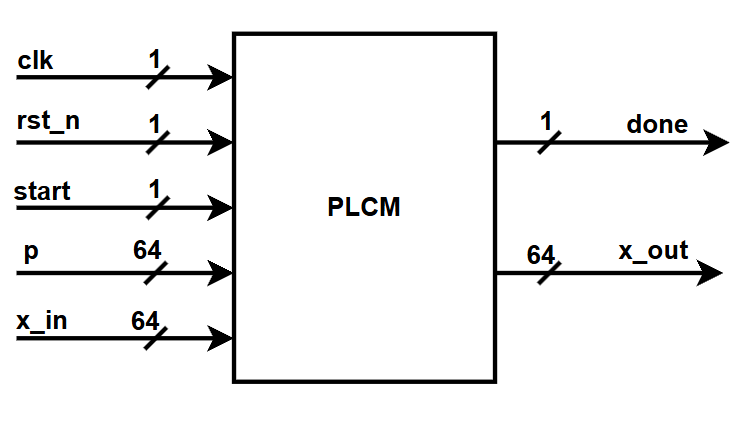
\includegraphics[width=0.8\textwidth]{Figures/plcm_io.png}
	\caption{Sơ đồ chân IO Khối plcm}
	\label{hinh_sodo_plcm}
\end{figure}

\textbf{Tổng quan tín hiệu vào/ra}

\begin{table}[H]
	\centering
	\caption{Bảng mô tả các tín hiệu giao tiếp ngõ vào/ra của khối plcm}
	\begin{tabular}{|c|c|c|c|c|p{5.5cm}|}
		\hline
		\textbf{Tín hiệu} & \textbf{Số bit} & \textbf{I/O} & \textbf{Reg/Wire} & \textbf{Mức hoạt động} & \textbf{Chức năng} \\ \hline
		clk             & 1  & I & Wire & Sườn lên & Tín hiệu đồng hồ đồng bộ. \\ \hline
		rst\_n          & 1  & I & Wire & Mức thấp & Đặt lại mạch và FSM về trạng thái IDLE. \\ \hline
		start           & 1  & I & Wire & Mức cao  & Kích hoạt một chu kỳ tính toán hệ hỗn loạn. \\ \hline
		p               & 64 & I & Wire & N/A      & Tham số điều khiển hỗn loạn (định dạng Q2.62). \\ \hline
		x\_in           & 64 & I & Wire & N/A      & Trạng thái hạt giống đầu vào (định dạng Q2.62). \\ \hline
		x\_out          & 64 & O & Reg  & N/A      & Trạng thái hỗn loạn kế tiếp sau phép tính. \\ \hline
		done            & 1  & O & Reg  & Mức cao  & Báo hiệu hoàn tất 1 nhịp và dữ liệu đã hợp lệ. \\ \hline
	\end{tabular}
	\label{bang_plcm_module}
\end{table}

\textbf{Lưu đồ thuật toán}

\begin{figure}[H]
	\centering
	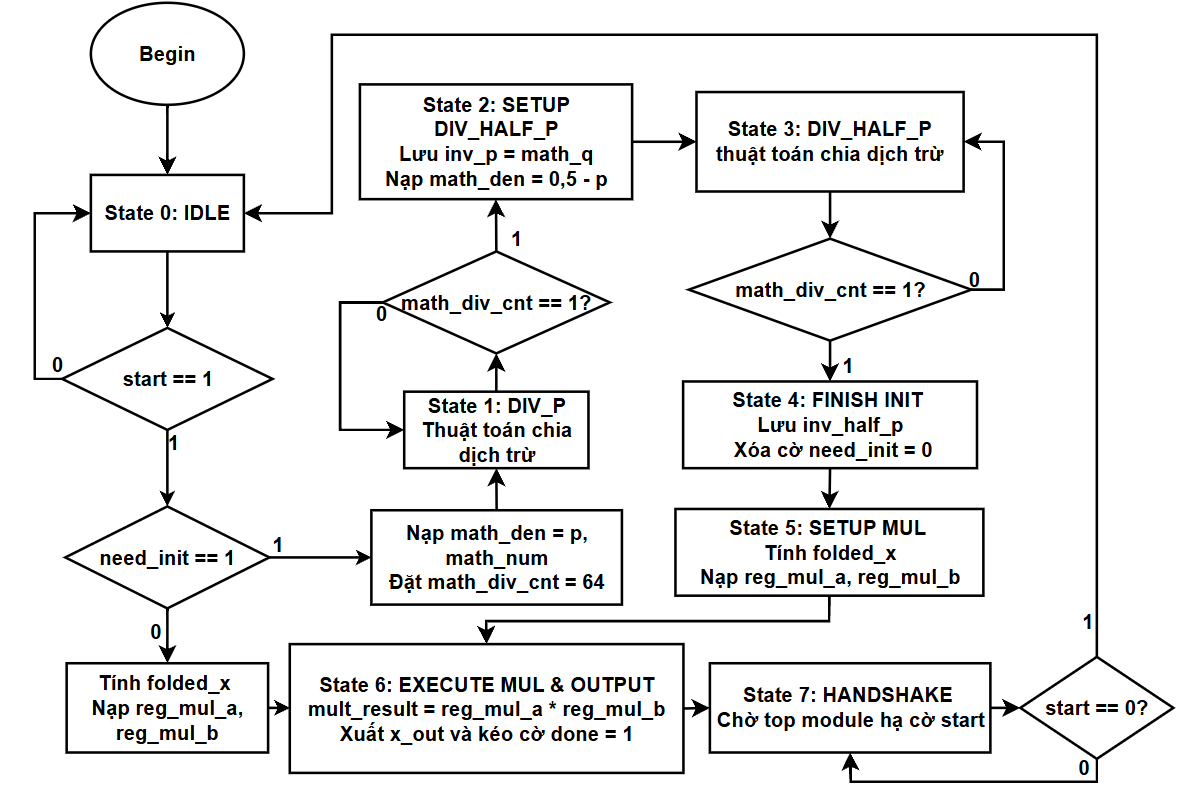
\includegraphics[width=1.0\textwidth]{Figures/plcm_sd.png}
	\caption{Lưu đồ thuật toán khối plcm}
	\label{fig:plcm_ld}
\end{figure}

\textbf{Giản đồ định thời}

\begin{figure}[H]
	\centering
	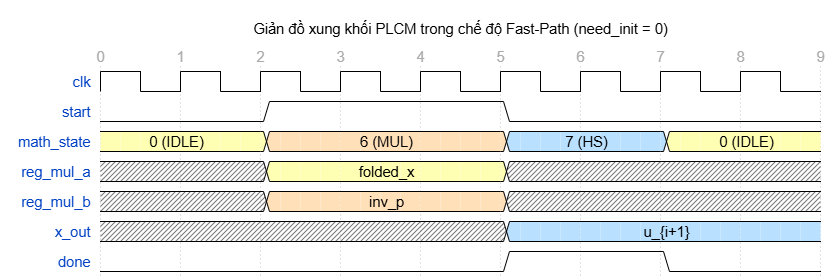
\includegraphics[width=1.0\textwidth]{Figures/plcm_td.png}
	\caption{Giản đồ định thời khối plcm khi need\_init = 0}
	\label{fig:plcm_f_td}
\end{figure}

\begin{figure}[H]
	\centering
	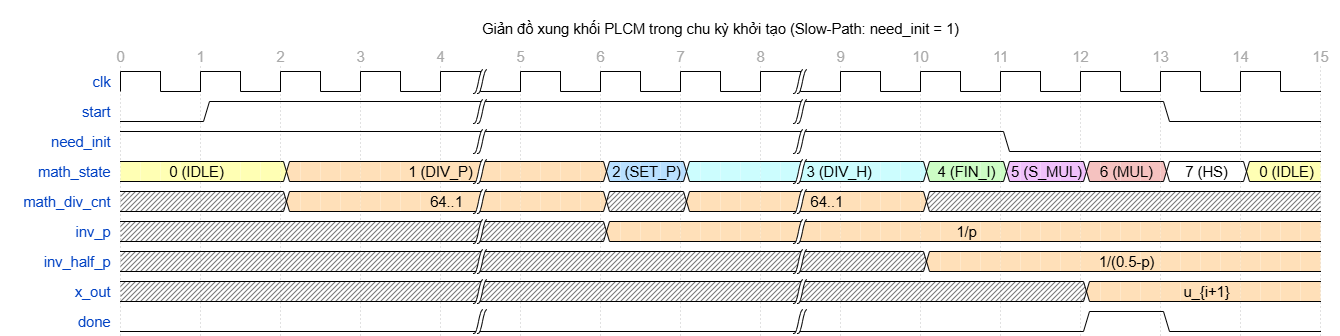
\includegraphics[width=1.0\textwidth]{Figures/plcm_sl_td.png}
	\caption{Giản đồ định thời khối plcm khi need\_init = 1}
	\label{fig:plcm_sl_td}
\end{figure}


\subsubsection{Khối confusion}
\textbf{Đặc tả chức năng hoạt động}

Khối \texttt{confusion} đảm nhận vai trò chuyên trách trong việc hoán vị dữ liệu thông qua thuật toán hỗn loạn Arnold's Cat Map. Quá trình xáo trộn không gian này đóng vai trò then chốt giúp phá vỡ hoàn toàn trật tự vị trí ban đầu của chuỗi byte, từ đó triệt tiêu các mối liên kết và đặc trưng thống kê hình học của luồng video nén chuẩn H.264. Nhằm tối ưu hóa thiết kế trên vi mạch FPGA, thay vì phải xây dựng các bộ dịch bit phức tạp để xử lý trực tiếp một chuỗi bitstream 1D có độ dài thay đổi liên tục, hệ thống phần cứng đã tự động ánh xạ và cuộn luồng 25 byte hệ số DC vào một không gian ma trận ảo có kích thước $5 \times 5$ để thực thi giải thuật một cách dễ dàng và hiệu quả hơn.

Nhằm nâng cao hiệu năng hoạt động của phần cứng đến mức tối đa, thiết kế đã chủ động loại bỏ và thay thế hoàn toàn phép chia lấy dư thông thường bằng một bảng tra cứu tổ hợp thông qua hàm \texttt{get\_mod5}. Kỹ thuật này giúp hệ thống giảm thiểu độ trễ tính toán xuống gần như bằng không mà không tiêu tốn thêm tài nguyên logic. Quan trọng hơn, nếu quyết định triển khai trực tiếp phép nhân ma trận hai chiều của Arnold's Cat Map theo cách truyền thống, hệ thống sẽ bị quá tải tài nguyên do phải sử dụng lượng lớn các bộ nhân tổ hợp, làm tăng mạnh độ trễ tới hạn. Phương trình hoán vị ma trận ban đầu có dạng:
$$ \begin{bmatrix} x' \\ y' \end{bmatrix} = \begin{bmatrix} 1 & p \\ q & 1+pq \end{bmatrix} \begin{bmatrix} x \\ y \end{bmatrix} \pmod 5 $$
Nhìn vào phương trình trên, biểu thức $1+pq$ đòi hỏi một khối nhân ma trận rất lớn và phức tạp. Để giải quyết triệt để vấn đề này, phương trình hoán vị đã được áp dụng kỹ thuật phân tách đại số, rã thành chuỗi hai phương trình tuyến tính một chiều. Trong cấu trúc mã Verilog, tọa độ $x$ tương ứng với chỉ số cột ($c$) và tọa độ $y$ tương ứng với chỉ số hàng ($r$). Ở chế độ mã hóa, trình tự tính toán được tối ưu lại như sau:
$$ x_{enc} = (c + p \cdot r) \pmod 5 $$
$$ y_{enc} = (r + q \cdot x_{enc}) \pmod 5 $$
Mạch logic tổ hợp sẽ ưu tiên tính toán chỉ số cột $x_{enc}$ ở tầng trước (\texttt{p\_mid}). Ngay khi có kết quả, hệ thống áp dụng kỹ thuật chuyển tiếp dữ liệu để đưa giá trị $x_{enc}$ này vào tiếp tục tính toán chỉ số hàng $y_{enc}$ ở tầng sau (\texttt{p3}). Giải pháp rã cấu trúc này giúp loại bỏ hoàn toàn bộ nhân phức tạp $1+pq$, giảm số lượng bộ nhân từ 4 xuống còn 2 mà vẫn duy trì được tốc độ thông lượng xử lý cực kỳ cao.

Tương tự đối với chế độ giải mã nghịch đảo, phương trình ma trận ngược nguyên thủy cũng gây ra những rào cản tài nguyên tương đương, đi kèm với nguy cơ sinh ra các tọa độ âm:
$$ \begin{bmatrix} x \\ y \end{bmatrix} = \begin{bmatrix} 1+pq & -p \\ -q & 1 \end{bmatrix} \begin{bmatrix} x' \\ y' \end{bmatrix} \pmod 5 $$
Hệ thống một lần nữa phân tách ma trận này, đảo ngược trình tự bằng cách tính toán chỉ số hàng $y_{dec}$ trước, sau đó mới tính chỉ số cột $x_{dec}$. Thêm vào đó, do kiến trúc phần cứng sử dụng chuẩn số nguyên không dấu, việc xuất hiện tọa độ âm là không hợp lệ. Để khắc phục triệt để, thiết kế đã chủ động cộng thêm hằng số bù 125 (một bội số của 5) vào từng biểu thức để dịch mốc tọa độ:
$$ y_{dec} = (r + 125 - q \cdot c) \pmod 5 $$
$$ x_{dec} = (c + 125 - p \cdot y_{dec}) \pmod 5 $$
Kỹ thuật bù giá trị này giúp hệ thống luôn duy trì được dải kết quả dương hợp lệ ở mọi chu kỳ tính toán, đồng thời hoàn toàn không làm thay đổi bản chất của phép toán đồng dư $\pmod 5$.

\textbf{Hoạt động của kiến trúc pipeline và giao tiếp I/O}

Giao diện vật lý của khối bao gồm các tín hiệu điều khiển vận hành cơ bản như nguồn xung nhịp \texttt{clk}, chân đặt lại \texttt{rst\_n}, cờ kích hoạt hệ thống \texttt{enable}, cờ chọn chế độ \texttt{mode} và các tham số hoán vị hình học \texttt{catmap\_p}, \texttt{catmap\_q} được truyền xuống từ bộ sinh khóa. Để tương tác trơn tru với hệ thống bộ nhớ trung tâm, khối sử dụng nhóm tín hiệu giao tiếp RAM tiêu chuẩn nhằm phát lệnh yêu cầu đọc dữ liệu nguyên bản và tiến hành ghi trả kết quả hệ số DC sau khi chúng đã bị xáo trộn vị trí.

Quá trình hoán vị ma trận được hệ thống vận hành trên một kiến trúc pipeline 4 tầng nhằm phân mảnh đường trễ và tối đa hóa thông lượng dữ liệu. Tại tầng thứ nhất, bộ đếm chuyên dụng sẽ quét địa chỉ tuyến tính từ 0 đến 24, từ đó mạch logic sẽ giải mã ra tọa độ hàng và cột của ma trận ảo để phát lệnh truy xuất bộ nhớ. Sang tầng thứ hai, hệ thống tạo ra một chu kỳ trễ đồng bộ để chờ đợi dữ liệu hệ số DC được trích xuất thành công từ mảng RAM nội bộ. Tầng thứ ba chính là phân hệ tính toán cốt lõi, nơi các mạch tổ hợp sẽ thực thi các phương trình biến đổi thuận hoặc nghịch đảo tùy thuộc vào trạng thái của tín hiệu \texttt{mode} để tìm ra tọa độ đích mới cho điểm ảnh. Ở tầng cuối cùng, khối sẽ tự động nội suy tọa độ vừa tìm được thành địa chỉ bộ nhớ thực tế và xác lập lệnh ghi để lưu đè an toàn byte dữ liệu vào vị trí mới đã bị xáo trộn. Quá trình đường ống này sẽ diễn ra liên tục, gối đầu nhau cho đến khi byte dữ liệu thứ 25 được hệ thống ghi thành công, lúc này khối sẽ phát ra xung cờ \texttt{done} để báo hiệu hoàn tất toàn bộ chu trình hoán vị.

\textbf{Sơ đồ chân IO}

\begin{figure}[H]
	\centering
	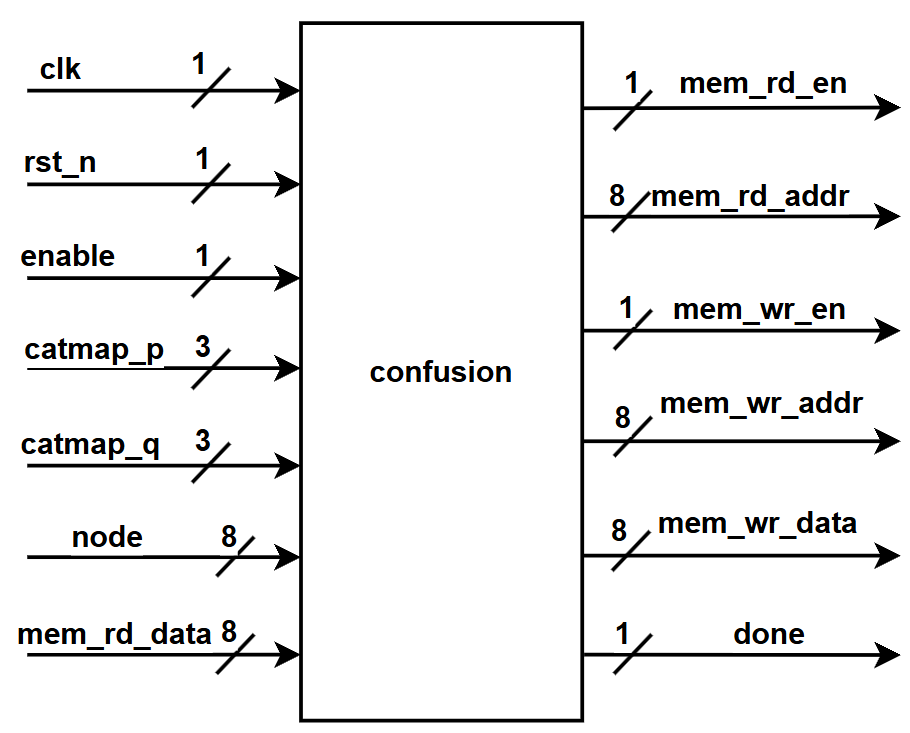
\includegraphics[width=0.5\textwidth]{Figures/conf_io.png}
	\caption{Sơ đồ chân IO khối confusion}
	\label{fig:conf_sd}
\end{figure}

\textbf{Tổng quan tín hiệu vào/ra}

\begin{longtable}{|c|c|c|c|c|p{4.5cm}|}
	\caption{Bảng mô tả các tín hiệu giao tiếp ngõ vào/ra của khối confusion}
	\label{bang_confusion} \\
	\hline
	\textbf{Tín hiệu} & \textbf{Số bit} & \textbf{I/O} & \textbf{Reg/Wire} & \textbf{Mức hoạt động} & \textbf{Chức năng} \\ \hline
	\endfirsthead
	
	\hline
	\textbf{Tín hiệu} & \textbf{Số bit} & \textbf{I/O} & \textbf{Reg/Wire} & \textbf{Mức hoạt động} & \textbf{Chức năng} \\ \hline
	\endhead
	
	\hline
	\endlastfoot

	clk             & 1 & I & Wire & Sườn lên & Nguồn xung nhịp hệ thống. \\ \hline
	rst\_n          & 1 & I & Wire & Mức thấp & Đặt lại hệ thống thanh ghi đường ống. \\ \hline
	enable          & 1 & I & Wire & Mức cao  & Kích hoạt bộ đếm để tiến hành đọc dữ liệu. \\ \hline
	catmap\_p       & 3 & I & Wire & N/A      & Tham số hoán vị $p$ của Arnold's Cat Map. \\ \hline
	catmap\_q       & 3 & I & Wire & N/A      & Tham số hoán vị $q$ của Arnold's Cat Map. \\ \hline
	mode            & 1 & I & Wire & N/A      & \texttt{0}: Mã hóa, \texttt{1}: Giải mã. \\ \hline
	mem\_rd\_en     & 1 & O & Wire & Mức cao  & Yêu cầu đọc byte dữ liệu nguyên bản từ RAM. \\ \hline
	mem\_rd\_addr   & 8 & O & Wire & N/A      & Địa chỉ quét tuyến tính chuỗi bitstream ($0 \rightarrow 24$). \\ \hline
	mem\_rd\_data   & 8 & I & Wire & N/A      & Dữ liệu hệ số DC nguyên bản phản hồi từ RAM. \\ \hline
	mem\_wr\_en     & 1 & O & Wire & Mức cao  & Yêu cầu ghi kết quả hoán vị vào RAM ngầm. \\ \hline
	mem\_wr\_addr   & 8 & O & Wire & N/A      & Địa chỉ mục tiêu (đã bị xáo trộn không gian). \\ \hline
	mem\_wr\_data   & 8 & O & Wire & N/A      & Dữ liệu hệ số DC được dịch chuyển tới vị trí mới. \\ \hline
	done            & 1 & O & Wire & Mức cao  & Báo hiệu hoàn tất tiến trình hoán vị khối 25 bytes. \\ \hline
\end{longtable}

\textbf{Lưu đồ thuật toán}

\begin{figure}[H]
	\centering
	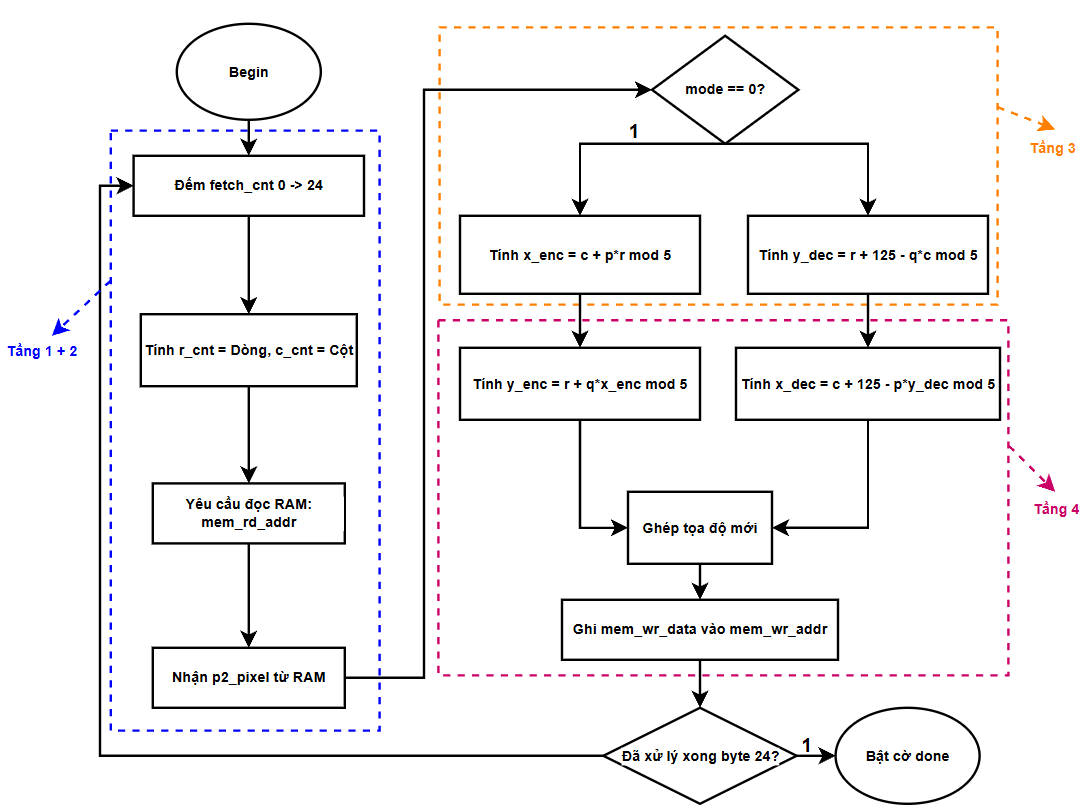
\includegraphics[width=1\textwidth]{Figures/conf_ld.png}
	\caption{Lưu đồ thuật toán khối confusion}
	\label{fig:conf_ld}
\end{figure}

\textbf{Timing diagram}

\begin{figure}[H]
	\centering
	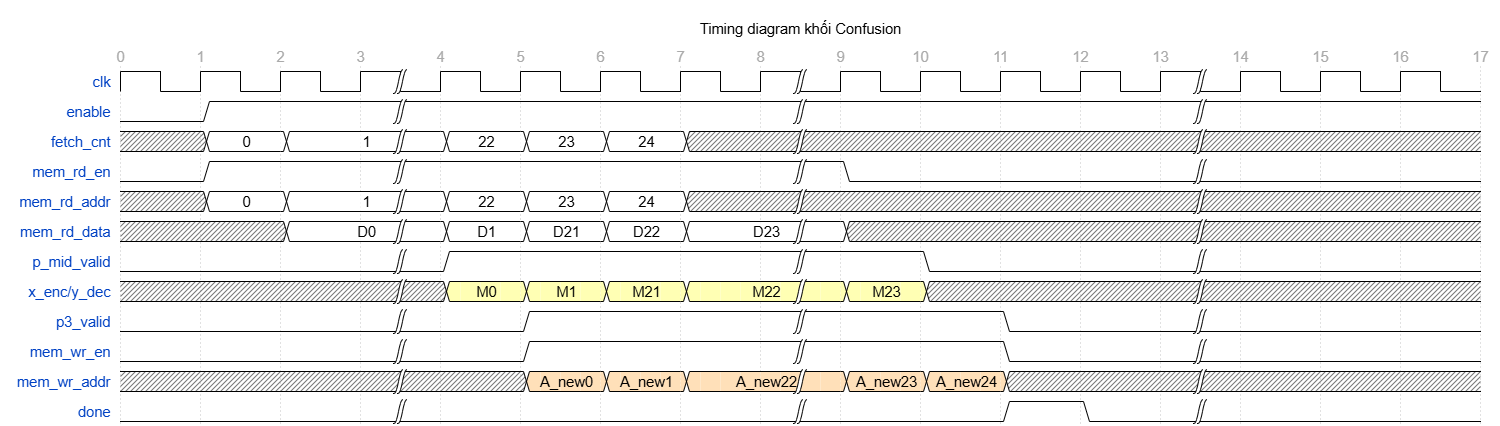
\includegraphics[width=1\textwidth]{Figures/confusion_td.png}
	\caption{Timing diagram khối confusion}
	\label{fig:conf_td}
\end{figure}

\subsubsection{Khối diffusion}
\textbf{Đặc tả chức năng hoạt động}

Khối \texttt{diffusion} đảm nhận vai trò khuếch tán giá trị dữ liệu, một khâu cực kỳ thiết yếu trong mật mã học hỗn loạn nhằm phá vỡ triệt để mọi mối quan hệ thống kê tuyến tính giữa bản rõ ban đầu và bản mã đầu ra. Cơ chế khuếch tán lan truyền này giúp hệ thống mật mã tạo ra hiệu ứng tuyết lở, qua đó hệ thống có thể chống lại các phương pháp tấn công vi sai và tấn công phân tích thống kê một cách vô cùng hiệu quả. Khối phần cứng thực thi việc biến đổi giá trị của từng byte dữ liệu dựa trên sự kết hợp đồng thời của ba yếu tố quan trọng: giá trị byte dữ liệu hiện tại, chuỗi khóa giả ngẫu nhiên được trích xuất từ mảng RAM chứa khóa, và trạng thái toán học của byte dữ liệu liền trước nó. Đối với trường hợp là phần tử đầu tiên của khối dữ liệu, một mầm khuếch tán \texttt{seed} an toàn sẽ được hệ thống nạp vào để làm giá trị khởi tạo thay thế cho byte liền trước.

Đặc biệt, để khắc phục điểm nghẽn cố hữu về mặt độ trễ của quá trình phản hồi trạng thái tuần tự, vốn yêu cầu byte sau phải chờ byte trước xử lý xong, khối đã được thiết kế tối ưu hóa theo kiến trúc đường ống 4 tầng (4-stage Pipeline). Nhằm giải quyết dứt điểm hiện tượng xung đột dữ liệu sinh ra khi byte dữ liệu thứ $i$ cần sử dụng kết quả tính toán của byte $i-1$ nhưng dữ liệu này chưa kịp ghi trả hoàn tất vào bộ nhớ RAM, thiết kế đã áp dụng triệt để kỹ thuật chuyển tiếp dữ liệu (Data Forwarding). Kỹ thuật này thiết lập một đường định tuyến tắt chạy qua mạng lưới mạch tổ hợp, đưa trực tiếp kết quả tính toán từ tầng ghi quay ngược lại nạp vào tầng thực thi ngay trong cùng một sườn xung nhịp. Nhờ có cơ chế này, luồng ống dữ liệu có thể hoạt động đồng bộ và liên tục gối đầu nhau mà không cần hệ thống phải chèn thêm bất kỳ chu kỳ chờ nào, giúp thông lượng toàn hệ thống luôn duy trì ở mức tối đa.

\textbf{Hoạt động của kiến trúc pipeline và giao tiếp I/O}

Về mặt giao tiếp vật lý, khối nhận tín hiệu kích hoạt \texttt{enable} từ module điều khiển mức trên, đi kèm với đó là giá trị mầm khuếch tán \texttt{seed} và cờ chọn luồng xử lý \texttt{mode}. Hệ thống giao tiếp đồng thời với mảng RAM dữ liệu để thực hiện đọc/ghi chuỗi hệ số DC và mảng RAM khóa để trích xuất ra các byte khóa giả ngẫu nhiên tương ứng với vị trí điểm ảnh. Để đảm bảo an toàn cho dữ liệu, ngay khi bị mất tín hiệu kích hoạt, đường ống sẽ tự động vô hiệu hóa toàn bộ quá trình nạp để ngăn ngừa các tín hiệu rác trôi nổi đi vào làm hỏng hệ thống.

Quá trình tính toán khuếch tán luân chuyển đồng bộ và nhịp nhàng qua 4 tầng thanh ghi đường ống. Tại tầng thứ nhất, bộ đếm địa chỉ sẽ quét tuần tự và xuất tín hiệu yêu cầu truy xuất dữ liệu từ các cổng giao tiếp RAM. Sang tầng thứ hai, hệ thống thực hiện chốt lại các byte hệ số DC và byte khóa giả ngẫu nhiên vừa được mảng RAM phản hồi để đảm bảo thời gian thiết lập an toàn. Tầng thứ ba là trung tâm thực thi toán học cốt lõi, nơi mạch tổ hợp đóng vai trò là một bộ ghép kênh khổng lồ để định tuyến dữ liệu chuyển tiếp. Nếu hệ thống đang hoạt động ở chế độ mã hóa, mạch sẽ tính toán giá trị khuếch tán dựa trên byte hiện tại, byte khóa và kết quả mã hóa của phần tử liền trước được trích xuất trực tiếp từ ngõ ra của tầng ghi đằng sau. Trong trường hợp hệ thống chuyển sang chế độ giải mã, mạch sẽ thực hiện phép biến đổi số học nghịch đảo sử dụng dữ liệu bản mã nguyên bản được lưu trữ trong thanh ghi. Cuối cùng, tại tầng thứ tư, hệ thống sẽ phát lệnh ghi kết quả vừa được tính toán xong vào lại bộ nhớ RAM, đồng thời mạch sẽ liên tục giám sát địa chỉ để kích hoạt xung cờ hoàn thành \texttt{done} ngay khi byte dữ liệu thứ 25 cuối cùng được xử lý trọn vẹn.

\textbf{Sơ đồ chân IO}

\begin{figure}[H]
	\centering
	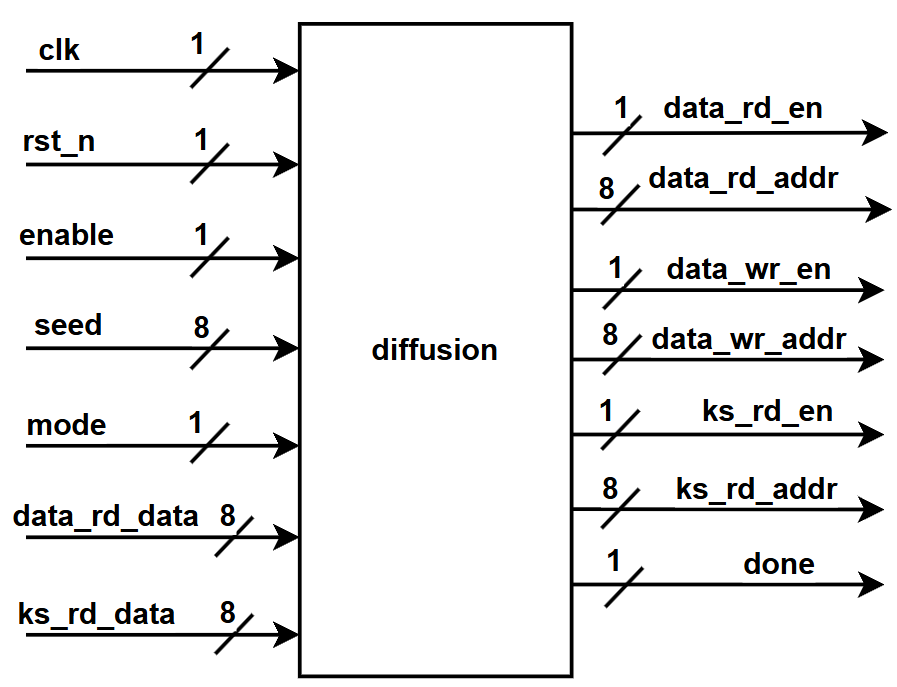
\includegraphics[width=0.9\textwidth]{Figures/diff_io.png}
	\caption{Sơ đồ chân IO khối diffusion}
	\label{fig:diff_sd}
\end{figure}

\textbf{Tổng quan tín hiệu vào/ra}

\begin{longtable}{|c|c|c|c|c|p{4.5cm}|}
	\caption{Bảng mô tả các tín hiệu giao tiếp ngõ vào/ra của khối diffusion}
	\label{bang_diffusion} \\
	\hline
	\textbf{Tín hiệu} & \textbf{Số bit} & \textbf{I/O} & \textbf{Reg/Wire} & \textbf{Mức hoạt động} & \textbf{Chức năng} \\ \hline
	\endfirsthead
	
	\hline
	\textbf{Tín hiệu} & \textbf{Số bit} & \textbf{I/O} & \textbf{Reg/Wire} & \textbf{Mức hoạt động} & \textbf{Chức năng} \\ \hline
	\endhead
	
	clk             & 1 & I & Wire & Sườn lên & Xung nhịp đồng bộ cấp cho pipeline. \\ \hline
	rst\_n          & 1 & I & Wire & Mức thấp & Đặt lại thanh ghi đường ống về trạng thái 0. \\ \hline
	enable          & 1 & I & Wire & Mức cao  & Kích hoạt nạp dữ liệu ở tầng truy xuất. \\ \hline
	seed            & 8 & I & Wire & N/A      & Giá trị mầm khuếch tán đầu vào. \\ \hline
	mode            & 1 & I & Wire & N/A      & \texttt{0}: Mã hóa, \texttt{1}: Giải mã. \\ \hline
	data\_rd\_en    & 1 & O & Wire & Mức cao  & Tín hiệu yêu cầu đọc hệ số DC từ RAM. \\ \hline
	data\_rd\_addr  & 8 & O & Wire & N/A      & Địa chỉ truy xuất byte dữ liệu cần xử lý. \\ \hline
	data\_rd\_data  & 8 & I & Wire & N/A      & Byte dữ liệu phản hồi từ RAM. \\ \hline
	data\_wr\_en    & 1 & O & Wire & Mức cao  & Tín hiệu yêu cầu ghi kết quả vào RAM. \\ \hline
	data\_wr\_addr  & 8 & O & Wire & N/A      & Địa chỉ ghi byte dữ liệu kết quả. \\ \hline
	data\_wr\_data  & 8 & O & Wire & N/A      & Byte dữ liệu kết quả sau khi khuếch tán. \\ \hline
	ks\_rd\_en      & 1 & O & Wire & Mức cao  & Tín hiệu yêu cầu đọc khóa từ RAM chứa khóa. \\ \hline
	ks\_rd\_addr    & 8 & O & Wire & N/A      & Địa chỉ truy xuất khóa ngẫu nhiên. \\ \hline
	ks\_rd\_data    & 8 & I & Wire & N/A      & Byte khóa ngẫu nhiên phản hồi. \\ \hline
	done            & 1 & O & Wire & Mức cao  & Báo hiệu hoàn tất vòng xử lý khuếch tán. \\ \hline
\end{longtable}

\textbf{Lưu đồ thuật toán}

\begin{figure}[H]
	\centering
	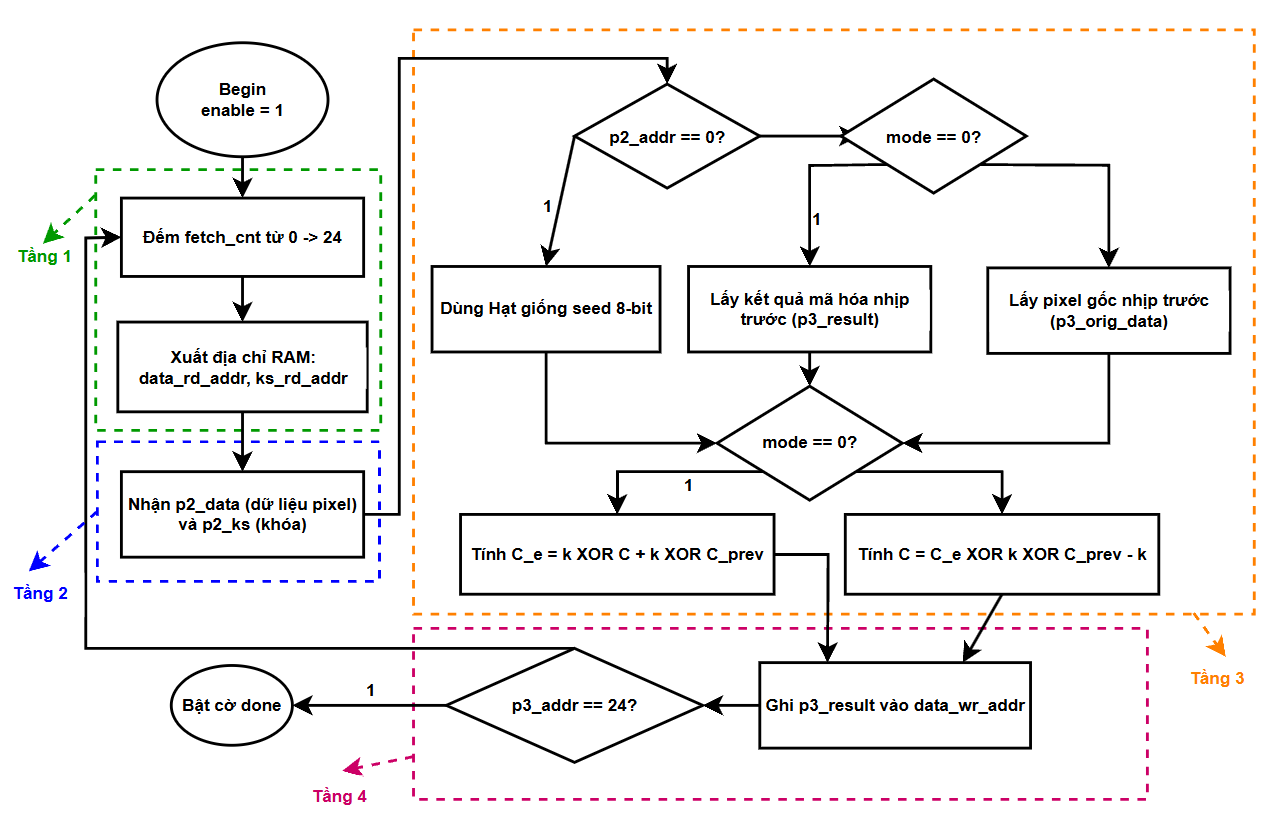
\includegraphics[width=1.0\textwidth]{Figures/diff_ld.png}
	\caption{Lưu đồ thuật toán khối diffusion}
	\label{fig:diff_ld}
\end{figure}

\textbf{Timing diagram}

\begin{figure}[H]
	\centering
	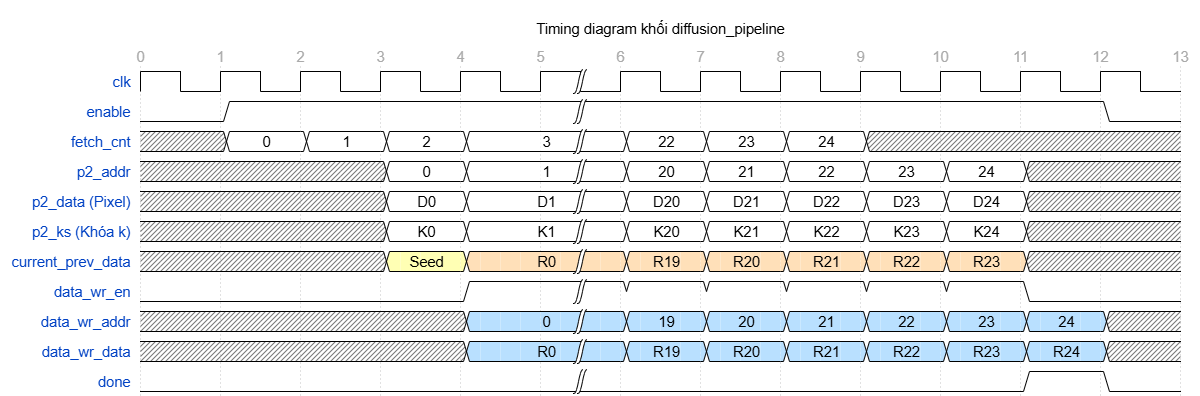
\includegraphics[width=1.0\textwidth]{Figures/diff_td.png}
	\caption{Timing diagram khối diffusion}
	\label{fig:diff_td}
\end{figure}

\subsection{Tổng kết chương 7}

Chương 3 đã đi sâu vào quá trình phân tích và thiết kế chi tiết kiến trúc phần cứng cho toàn bộ hệ thống mã hóa cũng như giải mã hỗn loạn. Thay vì tiến hành triển khai thuật toán theo cách nguyên thủy và rời rạc, thiết kế đã áp dụng một cách khoa học mô hình máy trạng thái kết hợp đường dẫn dữ liệu, tích hợp cùng với cơ chế định tuyến dữ liệu qua bộ nhớ trung tâm. Cấu trúc linh hoạt này đã chia tách rõ ràng các nhiệm vụ phức tạp giữa khối điều khiển trung tâm \texttt{crypto\_controller} và khối đường dẫn dữ liệu thụ động \texttt{crypto\_datapath}. Sự phân tách này không chỉ giúp quản lý hệ thống hiệu quả mà còn cho phép phần cứng tái sử dụng hoàn toàn các module toán học trong suốt các vòng lặp, từ đó tiết kiệm tối đa diện tích silicon trên vi mạch.

Xuyên suốt chương, từng phân hệ lõi của hệ thống đã được đặc tả một cách chi tiết, bắt đầu từ cơ chế hoạt động cốt lõi, sơ đồ kết nối I/O, cho đến lưu đồ thuật toán và giản đồ định thời tương ứng. Đặc biệt, đồ án đã chứng minh khả năng áp dụng thành công những kỹ thuật thiết kế vi mạch nhằm tối ưu hóa thông lượng và gỡ bỏ các rào cản về mặt tài nguyên phần cứng. Điển hình có thể kể đến như việc chuyển đổi phép chia thành phép nhân với nghịch đảo trong khối \texttt{plcm}, thay thế hoàn toàn phép chia lấy dư bằng bảng tra cứu tổ hợp ở khối \texttt{confusion}, và thiết lập khéo léo cơ chế chuyển tiếp dữ liệu để giải quyết hiện tượng xung đột đọc/ghi trong khối \texttt{diffusion}. Sự hoàn thiện ở cấp độ thanh ghi của các module này tạo nên một cơ sở phần cứng vững chắc để hệ thống sẵn sàng bước vào giai đoạn kiểm chứng chức năng và đánh giá hiệu năng toàn diện ở các phần tiếp theo.
\clearpage